%!TEX root = ../thesis.tex
%*******************************************************************************
%****************************** Third Chapter **********************************
%*******************************************************************************

% **************************** Define Graphics Path **************************
\ifpdf
    \graphicspath{{Chapter3/Figs/Raster/}{Chapter3/Figs/PDF/}{Chapter3/Figs/}}
\else
    \graphicspath{{Chapter3/Figs/Vector/}{Chapter3/Figs/}}
\fi

%*******************************************************************************
%****************************** Second Chapter *********************************
%*******************************************************************************

\chapter{The VIDARR Detector}\label{Chp:ThePrototypeDetector}
This chapter will discuss the Liverpool prototype and its upgrade to the VIDARR detector system. The initial basis for the detector, the T2K ND 280 (near detector at 280\,m) Electromagnetic Calorimeter (ECal) will also be covered. As well as a brief mention of the expected gamma energies and neutron rates at high powered research reactors. The upgrade progressed steadily until December 2019. Despite the ongoing uncertainty and disruption due to the COVID-19 pandemic the detector has had a $\sim$ 50\,\% increase in mass and new cooling system and new mobile container laboratory. At time of writing the electronics are currently being upgraded. 

\section{Technology And Results}
%This thesis will cover consider RMon and the upgraded detector VIDARR. RMon the original prototype detector was re-purposed technology from the T2K ND280 (Near Detector (at) 280\,m) Electromagnetic Calorimeter (ECal) \cite{Allan_2013}. The VIDARR detector uses the same detection media but upgraded electronics and containment which will be referred to as the VIDARR detector. This section will focus on the RMon detector.
This section will focus on the initial detector and so a look at the underlying technology of the prototype, the ND280 ECal, is required. The ND280 detector located at JPARC is part of the T2K experiment and is used to study the muon neutrino beam used for neutrino oscillation measurements. The T2K ND280 detector consists of a central sub detector comprised of a pi-zero detector furthest upstream from the beam which is constructed from solid plastic scintillator and water bags \cite{theT2kExperiment2011}. The water bags can be filled or emptied to determine the target-water cross-section, water is used as the ND280 is the near detector for super-K in the T2K experiment. Then the detector is interspersed with Time projection chambers (TPCs) fine-grained detectors (FGDs) are scintillating bars with alternating layers in the x-y and measured 9.61\,mm\,$\times$\,9.61\,mm\,$\times$\,1864.3\,mm \cite{theT2kExperiment2011}. These bars are comprised of the same scintillator as the VIDARR detector. The sub-detector array can operate at a maximum data rate of 20\,Hz. Therefore, when taking data at the maximum rate the time gate opens every 50\,ms and data is taken over 10\,$\mu$s \cite{theT2kFGDs2012}. These sub-detectors use lead as the interaction medium surrounded by ECals to stop and measure particles leaving the central detector (see figure \ref{fig:nd280Fig}). The ECals used lead sheets as a conversion material as well as a secondary target. The ECal scintillating bars are the only active detector element that VIDARR inherited from the T2K ND280 detector but a brief overview of the detector was given here for completeness sake. 
%\\\\As it is the basis for the other detectors a quick overview of the T2K ND280 ECal will be required. The ND280 is a series of detectors from the neutrino oscillation experiment T2K which relies on a $\nu_\mu$ beam entering the detector shown in figure \ref{fig:nd280Fig}. This detector was comprised of several different detectors including time projection chambers (TPCs) and fine-grained detectors (FGDs) and electromagnetic calorimeters (ECals) \cite{Allan_2013}. The ECals are of particular interest as they are the basis for the RMon and VIDARR detector due to their robust design inert nature and high precision.  

\begin{figure}[!h]
 \centering
 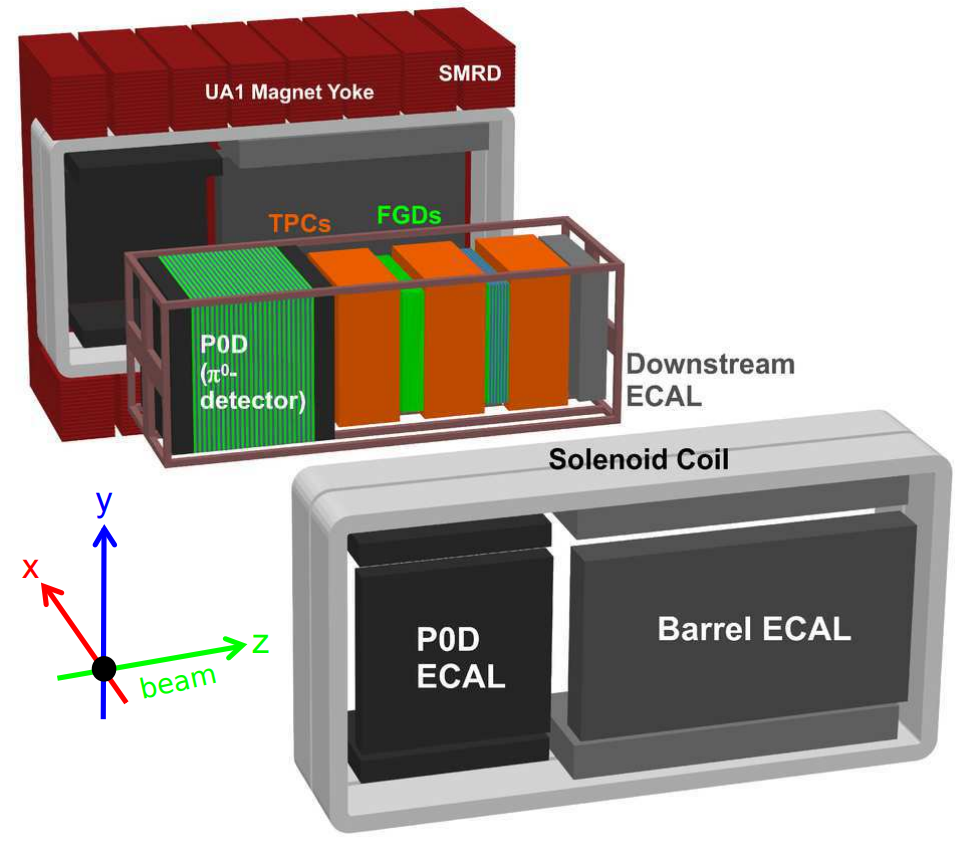
\includegraphics[width=\linewidth/2]{Chapter2/Figs/Raster/ND280Fig.png} 
 \captionof{figure}[Diagram of the ND280 detector.]{Diagram of the ND280 detector, the detector is based on the Barrel ECal. From \cite{Allan_2013}} %~can be used as a kind of place holder in latex
 \label{fig:nd280Fig}
\end{figure}

The T2K ECals are made from plastic scintillating bars measuring $4\,\textrm{cm}\times1\,\textrm{cm}$ with varying lengths arranged in alternating layers at 90 degrees to each other (see figure \ref{fig:vidarrDiagram}) forming a hodoscope \cite{Allan_2013}. Wavelength shifting (WLS) fibres were placed in the centre of the scintillating bars to measure light collection which shift the wavelength from blue ($\sim$~400\,nm) to green ($\sim$~510\,nm) to more effectively utilise the quantum efficiency of the sensors \cite{Allan_2013}. These wavelength shifting fibres are then connected to multi-pixel photon counters (MPPCs) which produce pulses of charge roughly proportional to the number of photons detected. This in turn is related to the energy deposited in the bar. This signal is then read in by Trip-T front-end electronic boards (TFBs) which integrates the charge received into an array of 23 time buckets of programmable width (480\,ns for ND280, 1.5\,$\mathrm{\mu}$s for the prototype). 
\\\\However, a crucial difference between the ECals of the ND280 and the VIDARR detector is that the lead sheets have been replaced with 1520\,mm\,$\times$\,1520\,mm\,$\times$\,0.2\,mm Mylar sheets which have been coated in Gadolinium oxide so that  neutrons produced in IBD (equation \ref{inverse_beta_decay}) are captured. The Mylar sheet coating was a polymer matrix mixed with white spirit. The original mixture had a ratio of 0.707 white spirit to 0.090 polymer matrix to 0.203 Gadolinium oxide. The white spirit is used to dissolve the gadolinium oxide and polymer matrix together. The resulting mixture is then applied via a spatula to the Mylar where the mixture dries out as the white spirit evaporates. The resulting sheets have a Gadolinium areal density of 12.8\,mg/cm$^2$ where 0.694 of the mixture left on the Mylar sheet is Gadolinium oxide. The detector was also designed to fit inside a shipping container with each bar having a length of 152\,cm and the active/instrumented volume measuring $152\,\textrm{cm}\times152\,\textrm{cm}$ with 49 layers of plastic scintillating bars giving a height of 49\,cm and a total of 1862 bars. The electronic systems were also adapted from the T2K ECal. They were reconfigured such that they were triggered by a neutron-induced gadolinium cascade from IBD by looking for a large number of hits in the trigger cycle. The ND 280 trigger (beam trigger) was changed into a ``look back'' trigger where of the 23 cycles 0 -- 17 are considered "prompt" and cycle 18 is the trigger cycle. Cycles 19 -- 22 were left as control so that they could be compared in case time-dependent issues arose from the altered system. As will be discussed later in chapter \ref{chp:cosmicMuonTomography}, cycles 19 -- 22 were used to diagnose a time dependant issue with the cosmic muon data set.
\\\\Electron anti-neutrinos  are detected by their absorption by a proton and decay into a positron and a neutron (see section \ref{subSec:IBD}). The positron and subsequent annihilation gamma-rays leave short tracks in the detector. The annihilation particles may be used to distinguish the positron from the beta decay electron backgrounds. In an IBD event the neutron is absorbed by the Gadolinium sheets in the detector which then causes an 8\,MeV gamma-ray cascade which will be expanded upon in section \ref{sec:GEANT4Simulation_modellingGadolinium}. Gadolinium is one of the most preferred neutron capture agents due to the higher energy gamma-rays and its extremely high capture cross-section of 48,890\,b \cite{Abdushukurov_2010}. 

\begin{figure}[!h]
\centering
  \centering
  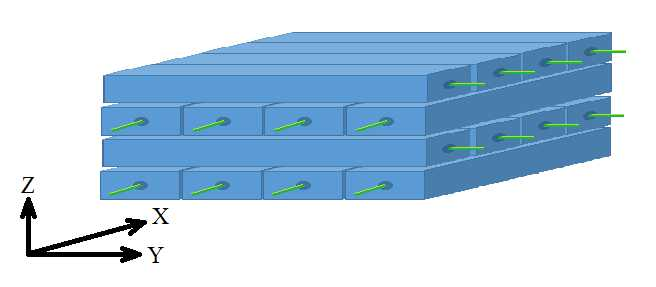
\includegraphics[width=0.6\linewidth]{Chapter2/Figs/Raster/VIDARR_diagram.jpeg}
  \captionof{figure}[A cutaway diagram showing the scintillator bar arrangement of the ND280 ECal and VIDARR]{A cutaway diagram showing the scintillator bar arrangement of the ND280 ECal and VIDARR detectors. The segments are 4\,cm wide $\times$ 152\,cm long $\times$ 1\,cm tall. The Gadolinium sheets in-between the VIDARR segments are not shown. From \cite{GeorgeHoltDiagram}.}
  \label{fig:vidarrDiagram}
\end{figure}

The detector was deployed at the Wylfa Magnox Power Station in Anglesey, Wales for an 18-month period. This run proved successful in measuring an increase in IBD candidate events which correlated with an increase in reactor power output. Figure \ref{fig:prototypeMeasumentFlux} compares the measured electron anti-neutrino flux with the reported power output and shows how good the agreement is. A measured anti-neutrino candidate rate of 172.1 $\pm$ 4.6 candidates per day is observed when the reactor is off and 203.7 $\pm$ 19.6 when the reactor is on \cite{Carroll_2018}. These results line up with the expectation from the SONGS1 deployment (figure \ref{subFig:reactorPowerSongsS1}) where a increase in electron anti-neutrino candidates correlates with an increase in reactor power. %Unfortunately due to cooling issues with the RMon detector the reactor shutdown was not observed. This is one of the main motivating factors behind the upgrade of the detector as the first generation MPPCs and repurposed electronics were susceptible to high levels of noise if the temperature was not carefully controlled. 
\begin{figure}[!h]
 \centering
 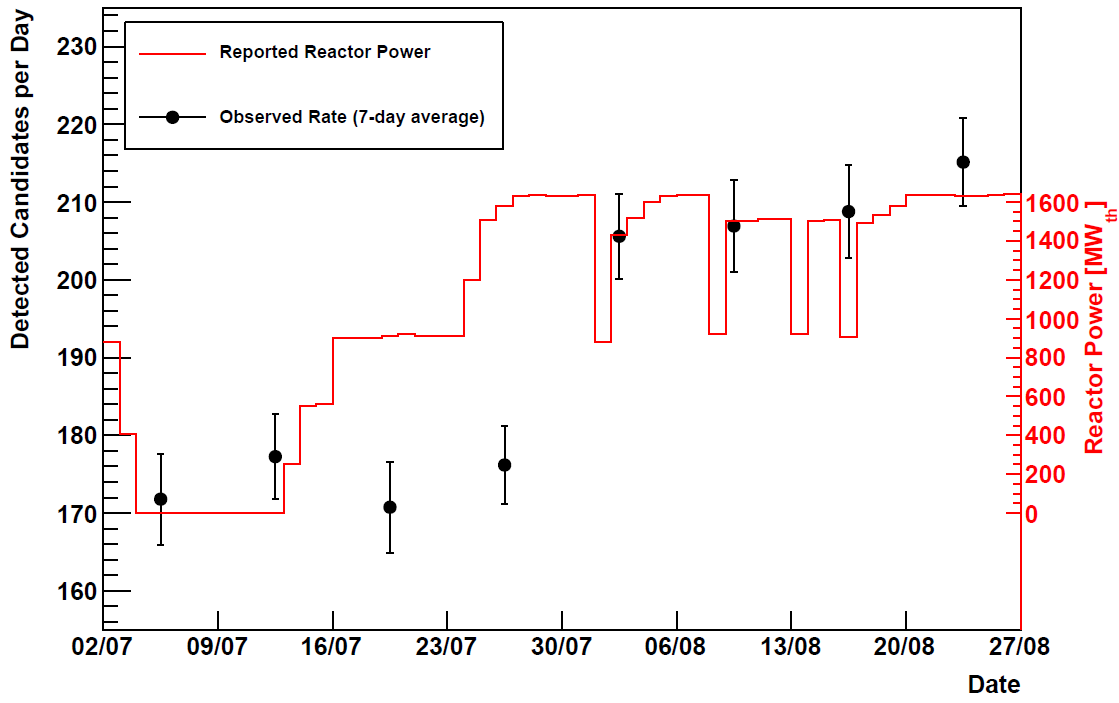
\includegraphics[width=0.7\linewidth]{Chapter2/Figs/Raster/prototypeMeasureOnFig.png} 
 \captionof{figure}[Measured anti-neutrino flux compared to the power generation from the Wylfa power station.]{Measured anti-neutrino flux compared to the power generation from the Wylfa power station for the prototype detector (49 layers). The increase in electron anti-neutrino candidates correlates with an increase in power generation. These results demonstrate the success of the prototype's deployment and technology. From \cite{Carroll_2018}} %~can be used as a kind of place holder in latex
 \label{fig:prototypeMeasumentFlux}
\end{figure}

Considering the re-purposed nature and rapid development cycle of the deployment at Wylfa and subsequent neutrino measurement (see figure \ref{fig:prototypeMeasumentFlux}) is a good demonstration of the detection media and experimental setup. However, whilst these results are highly encouraging, the response measurement can still be improved, for example the SONGS1 measurement is more accurate (see figure \ref{fig:reactorPowerAndRefuelingSongsS1}). In addition, the PANDA collaboration has been able to measure a neutrino energy spectrum the from Ohi power plant at a distance of $\sim$ 50\,m \cite{IIRIE_Panda_2021} (see figure \ref{subFig:Panda_spectrumOfIbdCandidates}). With an upgraded version of the detector it should be possible to achieve similar results to SONGS1 and PANDA and current modelling is ongoing to assess the nuclear waste measuring potential of VIDARR. 

\section{Background Measurements At Reactor Sites}
Backgrounds at reactor sites are important to quantify as it helps to guide shielding and understand irreducible backgrounds. The results from SONGS1, PANDA, and Wylfa all show low count rates per day of the order of a hundred events per ton of active detector mass. These low count rates necessitate a good understanding of background. The PROSPECT experiment has done a  study looking into the background at two research reactor locations, the National Bureau of Standards Reactor (NBSR) at NIST and the High Flux Isotope Reactor (HFIR) at ORNL \cite{Ashenfelter_2016}. Another site was considered by the PROSPECT collaboration, the ATR at INL but the increased altitude of that site leads to a significantly higher cosmogenic neutron flux \cite{Ashenfelter_2016}. An example of how reactors affect the background can be seen in figure \ref{fig:Prospect_NSBR_gammaSpec} which shows how the gamma-ray spectrum varies when the NBSR is on and off, it shows how the spectrum between 3\,MeV -- 9\,MeV is mostly dominated by reactor noise. However, the gamma ray flux will also depend largely on the distance to the reactor. For a detector the size of VIDARR ($\sim$~2.5\,Tonnes) the gamma-ray flux will likely be dominated by contamination. An investigation into the background gamma-ray flux for VIDARR is due to start once construction is complete. 
\\\\Another major background component is the neutron flux of the reactor which is shown by figure \ref{fig:prospectNeutronMap} for the HFIR location. Thermal neutrons are an issue for electron anti-neutrino detectors but should be somewhat negated through robust positron identification and accurate double coincident measurements. Another more important background is fast neutrons because they cause a false double coincident signal by potentially interacting with protons and then thermalising and being absorbed. The majority of the neutron background is likely to be cosmogenic in nature for a detector deployed $\sim$~50\,m standoff from the reactors as VIDARR will be as figure \ref{fig:prospectNeutronMap} shows the fast and thermal neutron rate drops rapidly as distance from the reactor is increased. Cosmogenic neutron background for HFIR for the far detector location for PROSPECT (15\,m--20\,m) gives $4.4\,\pm\,0.3$~$\times$~$10^{-3}$\,cm$^{-2}$\,s$^{-1}$ extrapolating this for VIDARR would give $\sim$~100 cosmogenically induced neutrons per second. The measurement of the cosmogenic neutron background has been done by JEDEC in 2006 \cite{JEDEC_2006} as well as PROSPECT in figure \ref{fig:Prospect_HFIR_NBSR_nearFarPlots} which shows similar rates at different locations this is unsurprising as this is largely a function of altitude more than any other factor \cite{Ashenfelter_2016}. 
\\\\Another type of background that is easy to mitigate (for VIDARR) but also extremely useful are cosmic muons. Cosmic muons have a large number of events of $\sim$ 119\,s$^{-1}$m$^{-2}$ according to the CRY library \cite{ieee_cry_2007}. Cosmic muons form the latter half of this thesis (chapters \ref{chp:DataAnalysisTechniques}, \ref{chp:cosmicMuTelescopes}, \ref{chp:cosmicMuonTomography}) and they will be expanded upon then. They are background for anti-neutrino events as they hit a large number of channels thus setting off the neutron triggers these experiments rely on. Conversely, their high energy and highly penetrating nature means only a simple detector is required to quantify their rate, PROSPECT for example used the cosmic muon telescope seen in figure \ref{fig:Prospect_MuonPaddels}. The segmentation of VIDARR allows them to reject cosmic muon background very effectively which results in a 95\,\% reduction of cosmic muons when simulating them in GEANT4. This is because cosmic muons can be reasonably approximated as straight line tracks which are more easily identified with finer segmentation. % (also see figure \ref{fig:CRY_rates}). These particles can be detected by very simple detector requiring only a series of paddles as seen in figure \ref{fig:Prospect_MuonPaddels}. This cosmic $\mu$ background is useful as they are highly penetrating particles tracks that can be approximated to be straight lines (later discussed in chapter \ref{chp:cosmicMuonTomography}). The range of angles incident cosmic $\mu$ posses make them useful for tomographic purposes as will be discussed in chapter \ref{chp:cosmicMuTelescopes}. %% The angles of incidence of cosmic $\mu$ can have many useful applications and as such these cosmic $\mu$ should not be excluded as mere noise as will be shown in section \ref{sec:cosmicMuTelescopes}.


\begin{figure}[!h]
\centering
\begin{minipage}{.45\textwidth}
  \centering
  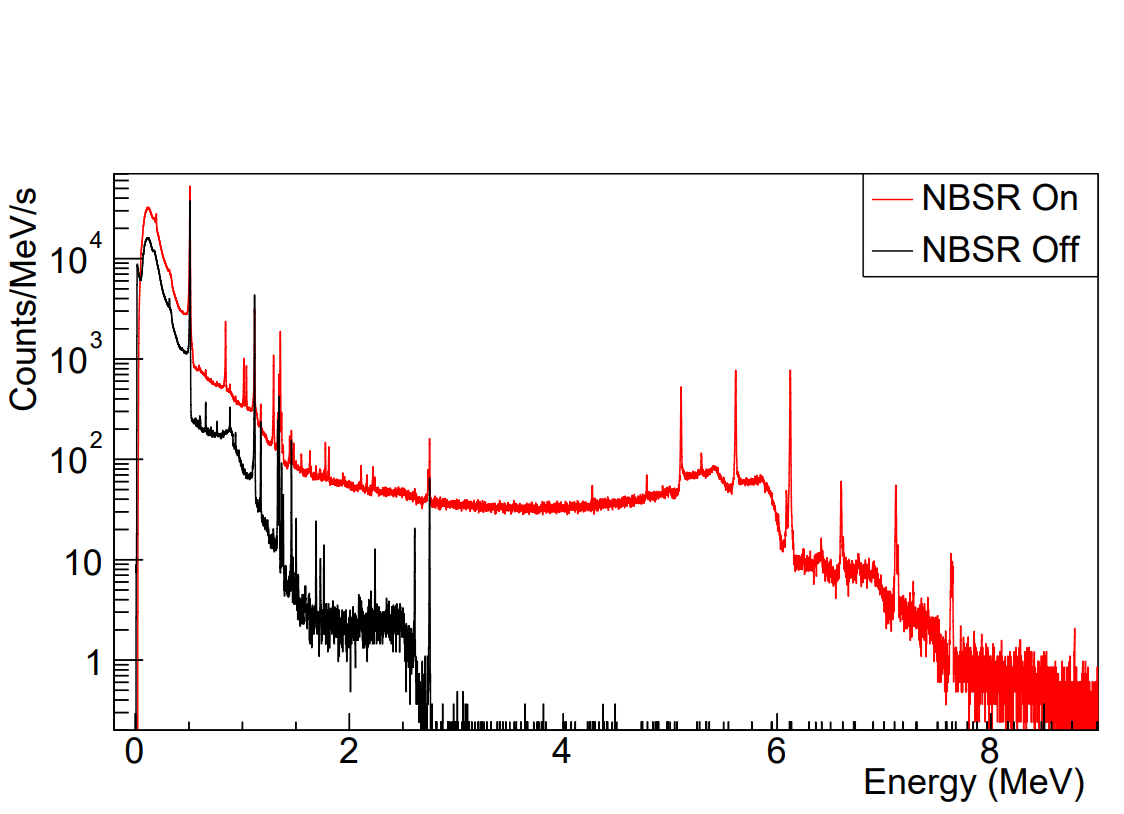
\includegraphics[width=\linewidth]{Chapter2/Figs/Raster/Prospect_NSBR_gammaSpec.png}
  \captionof{figure}[Example HPGe gamma-ray spectra taken with the NBSR on and off.]{Example HPGe gamma-ray spectra taken with the NBSR on and off. Prominent lines, and associated escape peaks and Compton continua, are evident. From \cite{Ashenfelter_2016} (table 2 in \cite{Ashenfelter_2016} shows line sources).} 
  \label{fig:Prospect_NSBR_gammaSpec}
  \vspace{1.912cm} %1 line = 0.478cm % 2 lines = 0.956cm % 3 lines= 1.434cm % 4 lines = 1.912cm % 5 lines = 2.39cm
\end{minipage}%
\qquad
\begin{minipage}{.45\textwidth}
  \centering
  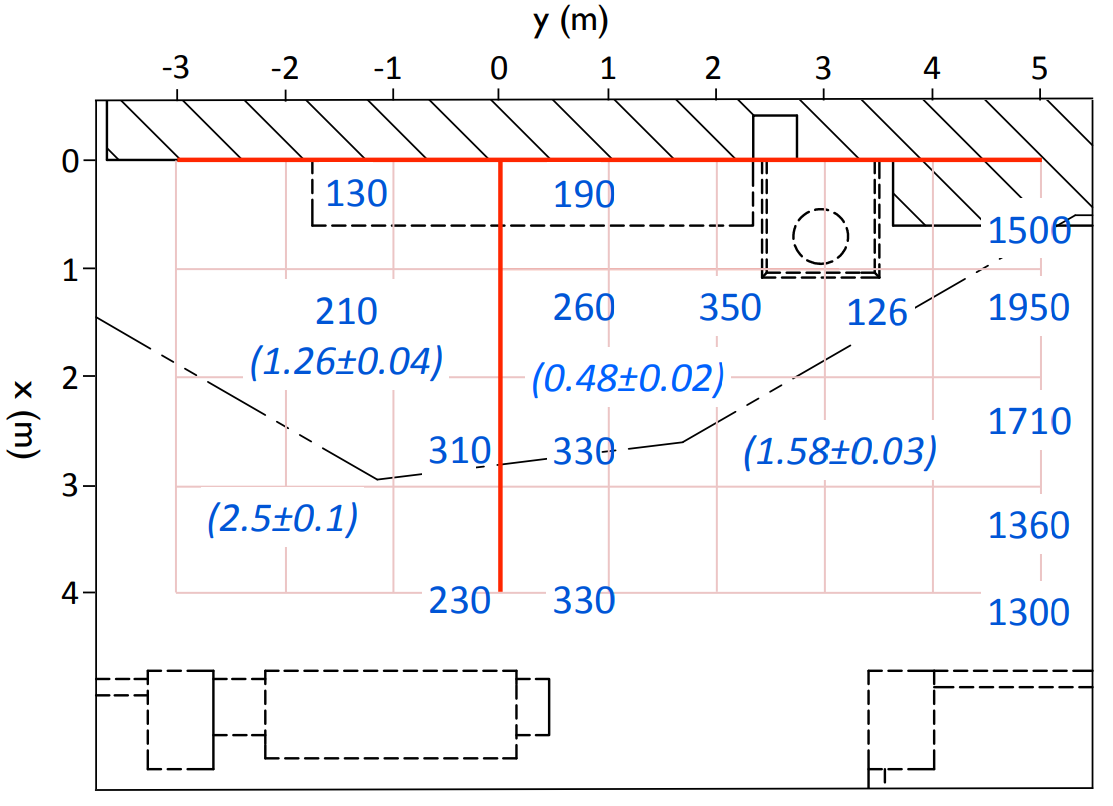
\includegraphics[width=\linewidth]{Chapter2/Figs/Raster/prospectNeutronMap.png} 
  \captionof{figure}[A pictorial representation of neutron dose rates at the HFIR near location.]{A pictorial representation of neutron dose rates (measured in nSv/h) and thermal neutron rates in italics (cm$^{-2}$ s$^{-1}$) at the HFIR near location (5\,m~--~10\,m standoff) roughly 15\,cm (z = 0.15) above the floor. Measurements are plotted on a one meter square grid referenced to the reactor wall (x = 0) and the smallest baseline (y = 0). The reactor core is centred at (x,y,z) = (-4.06,0,-3.85). From \cite{Ashenfelter_2016}.}
  \label{fig:prospectNeutronMap}
\end{minipage}
\end{figure}

% \begin{figure}[!h]
%  \centering
%  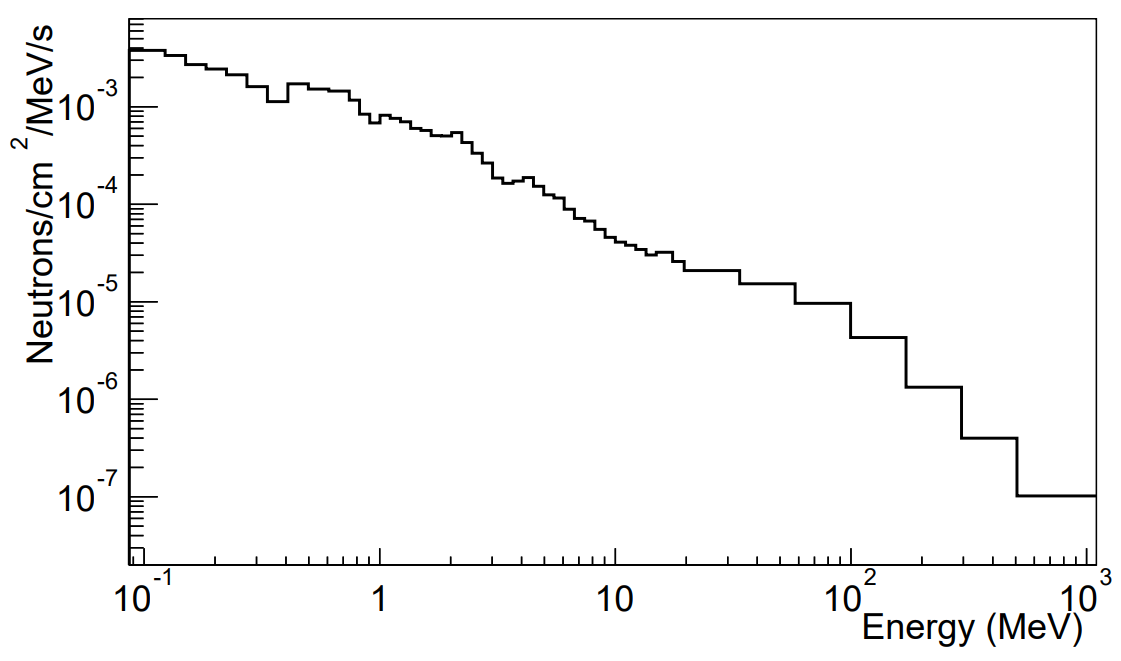
\includegraphics[width=0.7\linewidth]{Chapter2/Figs/Raster/JDEC_neutronSpec.png}
%  \captionof{figure}{The JEDEC standard fast neutron spectrum recorded at sea
% level in New York. From \cite{JEDEC_2006}. } 
%  \label{fig:JDEC_neutronSpec}
% \end{figure}

\begin{figure}[!h]
\centering
\begin{subfigure}{.5\textwidth}
  \centering
  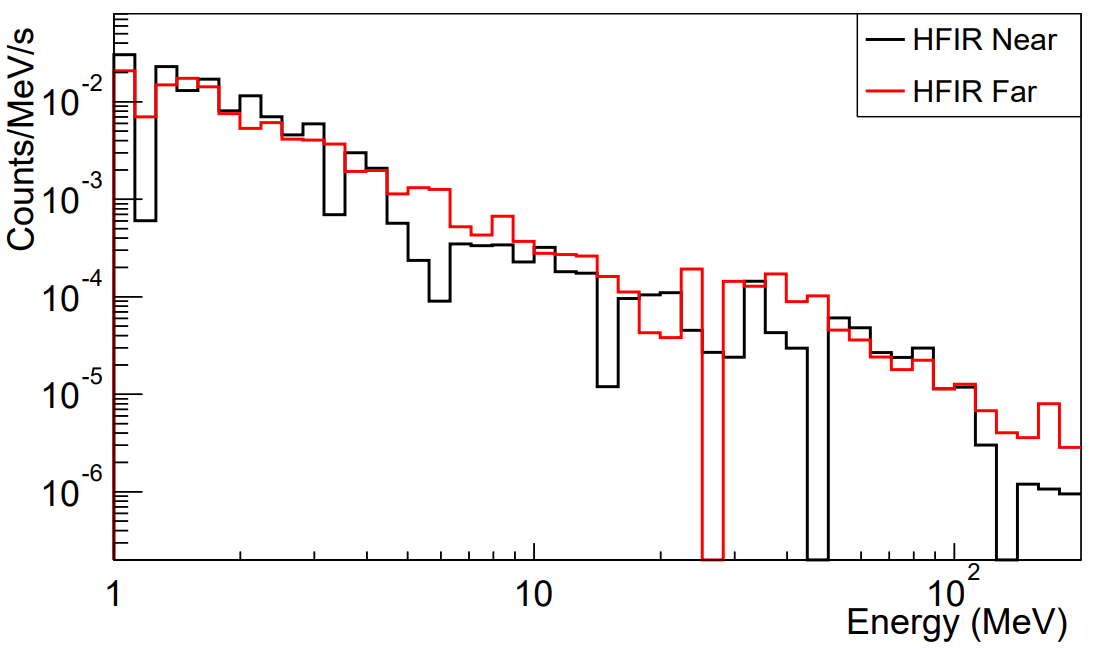
\includegraphics[width=\linewidth]{Chapter2/Figs/Raster/Prospect_HFIR_nearFarPlot.png}
  \captionsetup{width=.9\linewidth}
  \caption{}
  \label{subFig:Prospect_HFIR_nearFarPlot}
\end{subfigure}%
\begin{subfigure}{.5\textwidth}
  \centering
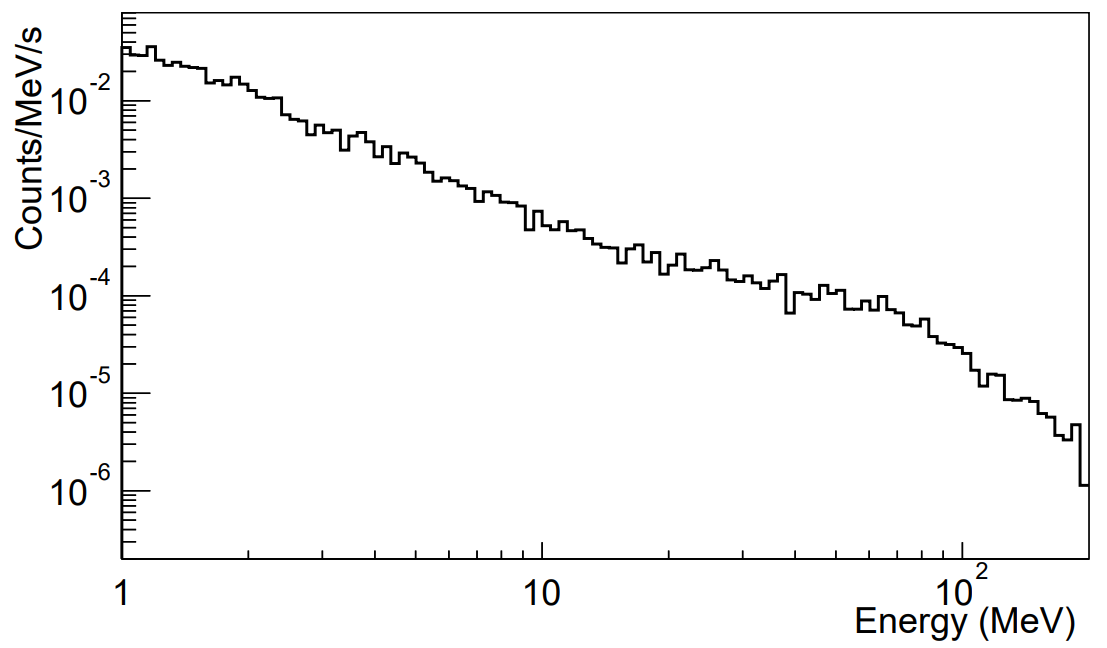
\includegraphics[width=\linewidth]{Chapter2/Figs/Raster/Prospect_NBSR_farPlot.png}
  \captionsetup{width=.9\linewidth}
  \caption{}
  \label{subFig:Prospect_NBSR_farPlot}
\end{subfigure}
\caption[The cosmogenic neutron-induced energy spectrum at HFIR and NBSR.]{The cosmogenic neutron-induced energy spectrum was recorded at the (a) HFIR near and far locations and (b) NBSR far location. From \cite{Ashenfelter_2016}.}
\label{fig:Prospect_HFIR_NBSR_nearFarPlots}
\end{figure}

\begin{figure}[!h]
 \centering
 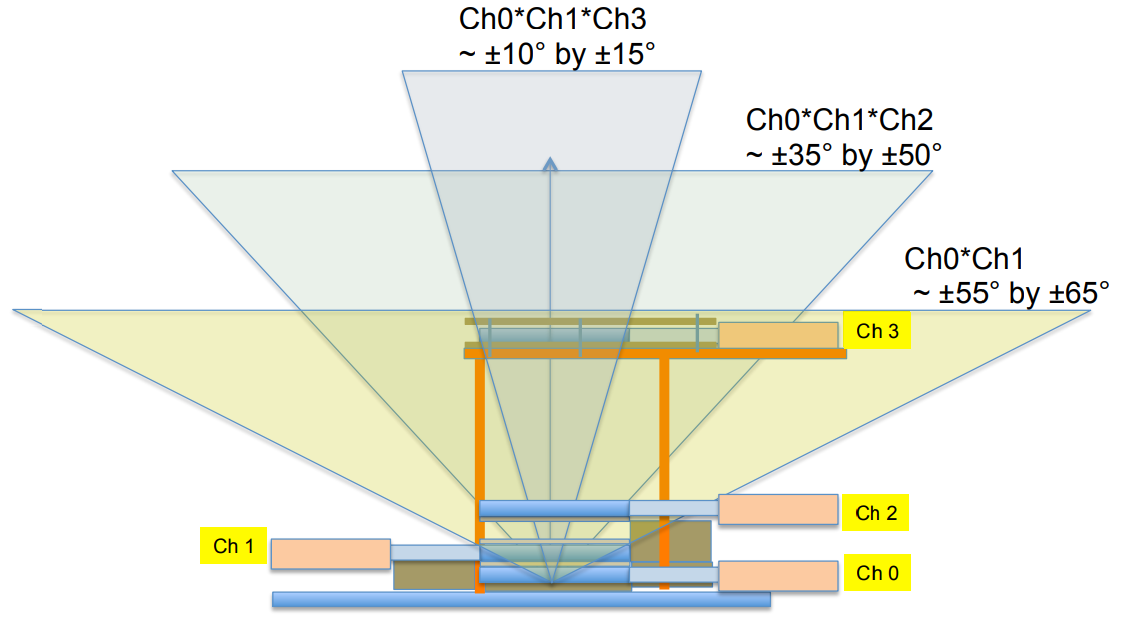
\includegraphics[width=0.7\linewidth]{Chapter2/Figs/Raster/Prospect_MuonPaddels.png}
 \captionof{figure}[Angular acceptances for a basic muon telescope.]{The angular acceptances for the muon telescope instrument used at all sites is determined by the coincidence requirement enforced between the 4 plastic scintillator paddles. These detectors were deployed by the PROSPECT experiment at both the NBSR and HFIR sites. From \cite{Ashenfelter_2016}.} 
 \label{fig:Prospect_MuonPaddels}
\end{figure}

%\clearpage
%white space
%\vspace{3cm}
\clearpage
\section{The VIDARR Detector Upgrade}\label{sec:theUpgradedDetector}
The deployment at Wylfa demonstrated that the choice of detector technology (scintillating bars, Gd doped sheets and light captured by WLS fibres) worked well. However, the detector would benefit from more active mass, higher efficiency sensors and dedicated electronics. The upgraded detector will have 21 more layers than the initial detector going from 49 to 70 layers and the additional 3 columns on side A are also now instrumented (see figure \ref{fig:detectorUpgradedmassOutlined}). This means the number of channels has increased from 1793 to 2660 which results in a mass increase of $\sim$ 50\,\%, thus improving the fiducial volume of the detector. The increase in layers will increase the average containment of the 8\,MeV Gd cascade in the detector allowing for more effective background reduction when triggering. The MPPCs are also a new generation with twice the efficiency going from ECal to VIDARR. %The increase in layers will not yield a significant increase in $e^+$ efficiency as $e^+$s are effectively contained to a $\sim$ 99\,\% level with both 1793 channels and 2660 channels as they are contained within 1-2 bars.

\begin{figure}[!h]
 \centering
 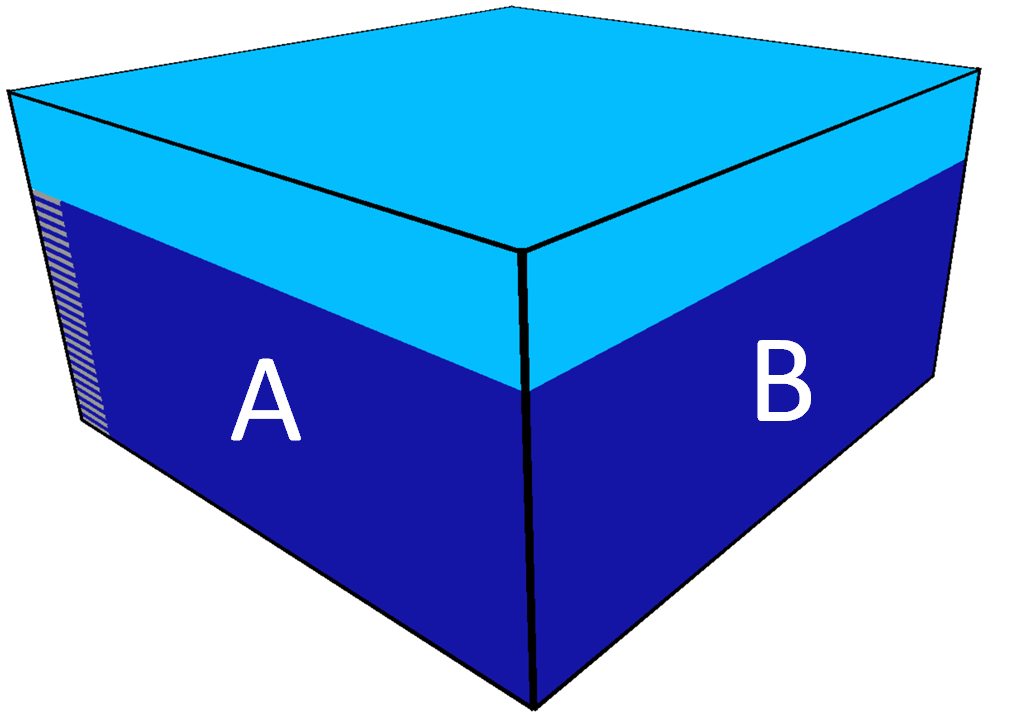
\includegraphics[width=0.5\linewidth]{Chapter3/Figs/detectorModelLabelled.png}
 \captionof{figure}[3d representation of the VIDARR detector upgrade.]{3D representation of the detector upgrade. The upgraded detector mass (light blue) is on top of the original mass (dark blue). The greyed out channels on the left hand side of side A were those left un-instrumented in the original deployment but are now instrumented in the upgrade.} 
 \label{fig:detectorUpgradedmassOutlined}
\end{figure}

The electronics have been improved significantly when compared to the original detector. The original electronics and sensors were taken from the T2K ECal. The MPPCs were the first generation of this technology with relatively low efficiency and high noise rates compared to the current generation used in the VIDARR detector. The energy resolution of the detector has been greatly improved by using more modern, higher efficiency MPPCs. In addition, the upgraded detector will have channel by channel trigger output to Field-Programmable Gate Array (FPGA) boards that connect with analogue boards in turn connecting to the MPPCs. The use of FPGA boards will allow for more complex trigger functions to be used and trigger on the detector as a whole (as opposed to the initial prototype's trigger which considered specific regions of the detector). This will be achieved by looking at the summed energy and the number of bars hit above each threshold. As will be expanded upon later in section \ref{sec:MachineLearningTrigger}, the improvement to energy resolution has a significant effect on the S/N ratio as well. During the analysis the lowest available threshold of $\sim$ 0.1\,MeV was the most effective in distinguishing signal from noise. This improvement is only possible due to the upgraded sensors and electronics. Both generations of MPPCs are highly temperature sensitive, and this did cause stability issues for the detector. %The use of two thresholds as opposed to one on the RMon also proved useful for improving generated neutron efficiency. 
%\\\\A basic cut investigation used a form of machine learning called a support vector machine (SVM) to determine the best cut and which dimensions gave the best separation. The cut was dominated by the number of bars hit at the lower threshold of 0.1\,MeV, the most accurate cut would have been utilising the number of bars hit above 0.1\,MeV and the summed energy above the 0.1\,MeV threshold. However due to the structure of the FPGA boards and their programming it was more prudent to use the number of bars hit above both the 0.1\,MeV thresholds and 0.5\,MeV threshold. The cost in classifier accuracy was minimal and it allowed for faster development of the FPGA firmware. 
\\\\To lessen temperature fluctuations in the upgraded VIDARR detector the cooling in and around the detector module has been greatly improved from the prototype. The prototype had six radiator fins on 2 sides of the detector which were primarily aimed at cooling the TFBs on each fin (see figure \ref{fig:detCon002_OldTearAway}). The upgraded VIDARR detector will also have cooling fins which will take heat away from the new boards but on the same 2 sides as the fins, there will also be two new radiators behind the fins which run the width and height of a side. The new active cooling the radiators will provide cooling to the cavity housing to the MPPCs and insulate them from heat generated by the active electronics. Further, the detector is now isolated from the readout computers and power supply units in a separate compartment in order to increase temperature stability. All of these improvements will allow for a more consistent temperature and reduce dark noise from the MPPCs below the original detector's levels. In addition temperature monitoring has also been added to ensure the MPPCs are maintained at the correct temperature.

\section{Detector Construction}\label{sec:DetectorConstruction}
In December of 2018, the original detector was moved out of the shipping container which housed it (figure \ref{fig:detCon000_TakeOut1}). It was then placed inside an ISO class 7 cleanroom, opened and disassembled (figure \ref{fig:detCon002_OldTearAway}). The prototype detector had reserved space that could be further utilised. The internal space of the shell was filled with 1\,m long cables connecting the sensors to the electronics, which were excess in length, (see figure \ref{fig:detCon002_OldTearAway}) and polystyrene filler in lieu of the top 21 layers. For VIDARR, the space inside the shell would be more efficiently utilised allowing for more electronics, sensors, and scintillator. The new scintillator purchased from Fermilab was more than twice as long as required and so was cut (see figure \ref{subFig:detCon003bb_CuttingScint}) so its dimensions matched the old scintillating bars ($152\,\textrm{cm} \times 4\,\textrm{cm} \times 1\,\textrm{cm}$). Once this was done, the edges of the freshly cut scintillator were arranged and painted with TiO$_2$ paint (figure \ref{subFig:detCon005b_PaintingEnds}) to reduce light losses at the end of the bar. The cut and painted scintillating bars were then placed inside the housing for the detector whilst it was in the cleanroom environment to minimise contamination (figure \ref{fig:detCon006_RonInCleanRoom}). The layers of scintillator have a white sheet of Mylar coated with Gadolinium oxide in between them, the reflective white sheet can be seen in figure \ref{fig:detCon006_RonInCleanRoom}, the Gadolinium oxide is necessary for capturing neutrons produced during IBD (section \ref{subSec:IBD}). 

\begin{figure}[!h]
\centering
\begin{minipage}{.45\textwidth}
  \centering
  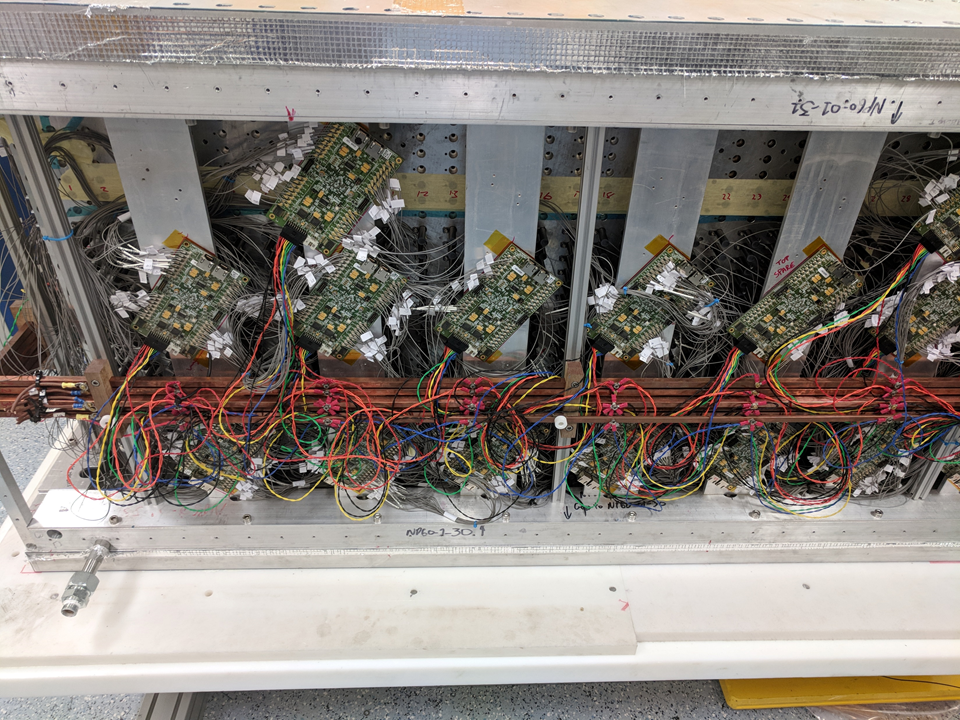
\includegraphics[width=\linewidth]{Chapter3/Figs/Raster/detCon002_OldTearAway.png}
  \captionof{figure}[A view of the electronics in the initial detector.]{A view of the electronics in the initial detector. There is much available space between the boards and the detector itself. The cables are 100\,mm long.} 
  \label{fig:detCon002_OldTearAway}
\end{minipage}%
\qquad
\begin{minipage}{.45\textwidth}
  \centering
  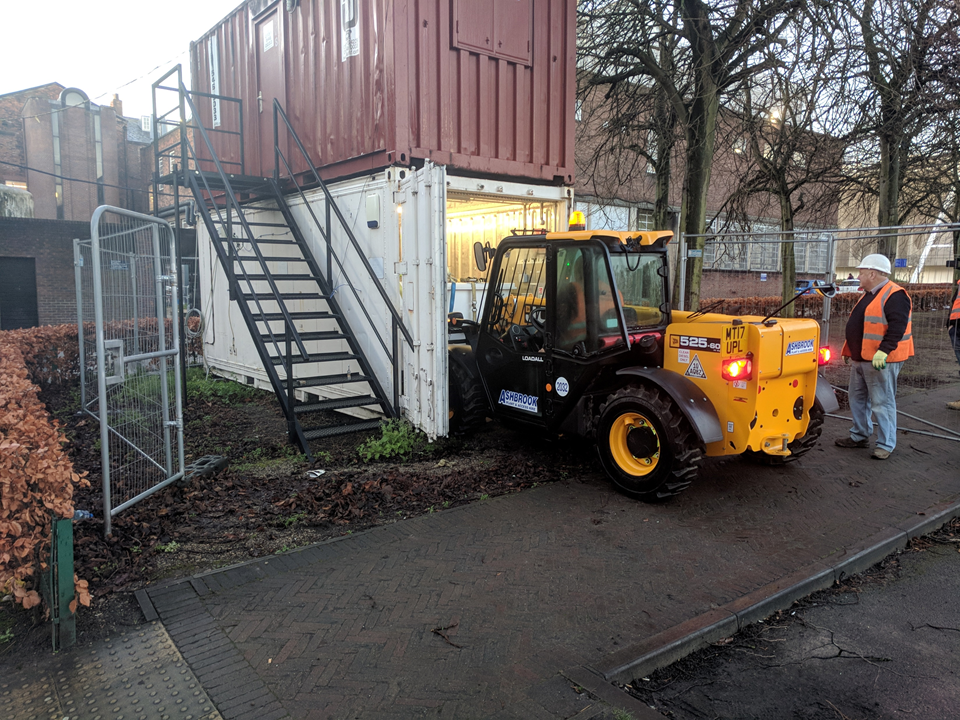
\includegraphics[width=\linewidth]{Chapter3/Figs/Raster/detCon000_TakeOut1.png} 
  \captionof{figure}[The detector being taken out of the original shipping container.]{The detector being taken out of the original shipping container which was a cooled standard shipping container.}
  \label{fig:detCon000_TakeOut1}
  \vspace{0.478cm} %1 line = 0.478cm % 2 lines = 0.956cm % 3 lines= 1.434cm % 4 lines = 1.912cm % 5 lines = 2.39cm
\end{minipage}
\end{figure}

\begin{figure}[!h]
\centering
\begin{subfigure}{.5\textwidth}
  \centering
  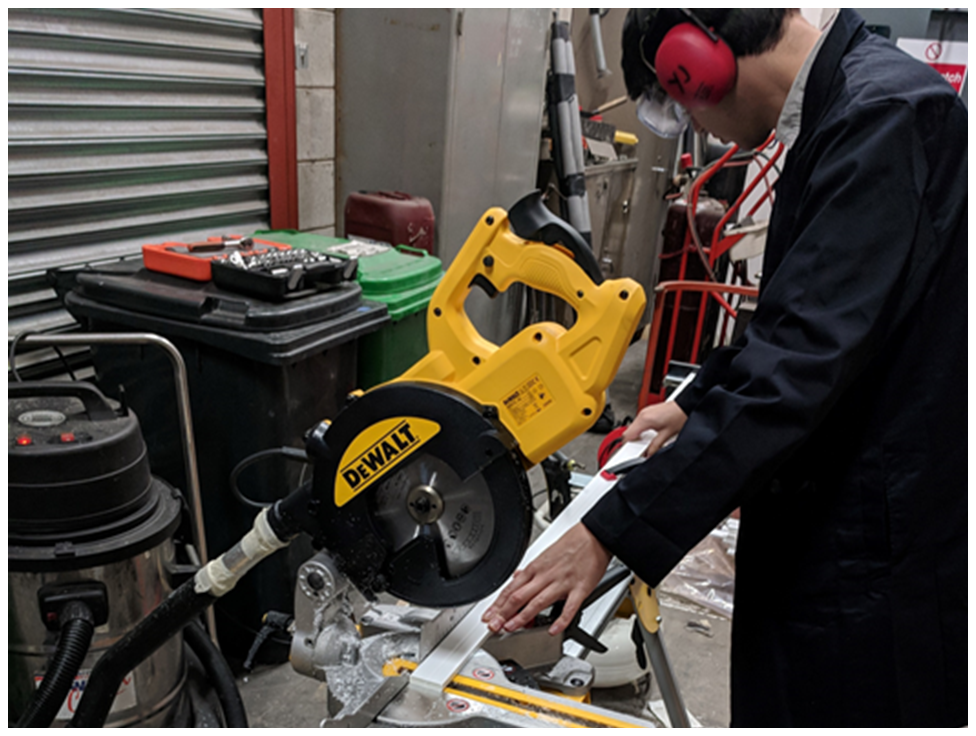
\includegraphics[width=\linewidth]{Chapter3/Figs/Raster/detCon003bb_CuttingScint.png}
  \captionsetup{width=.9\linewidth}
  \caption{}
  \label{subFig:detCon003bb_CuttingScint}
\end{subfigure}%
\begin{subfigure}{.5\textwidth}
  \centering
  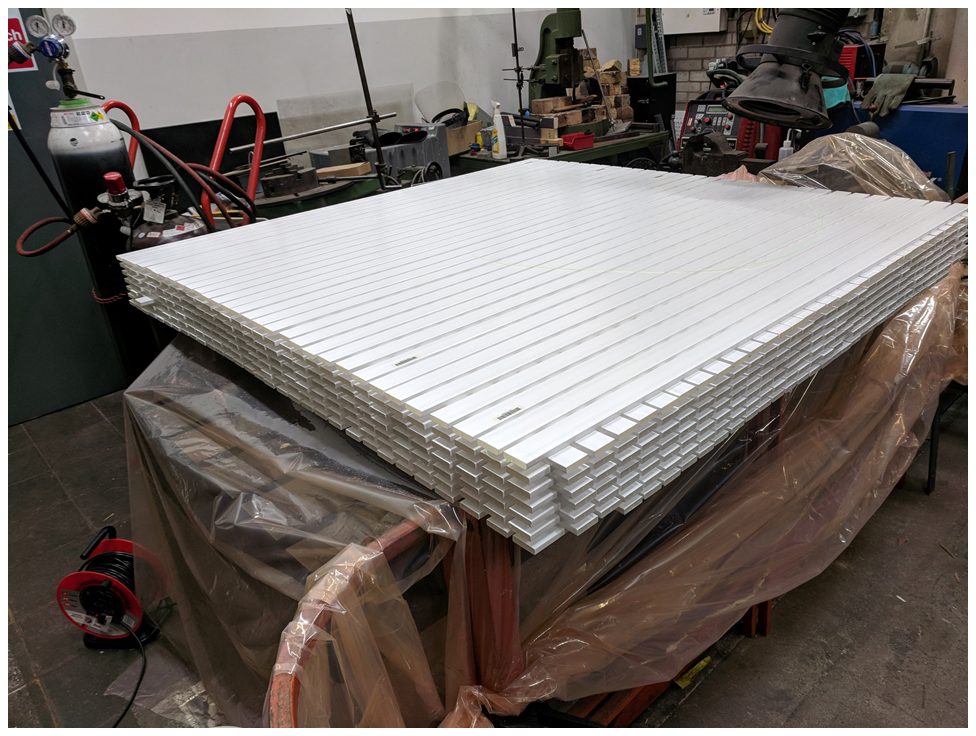
\includegraphics[width=\linewidth]{Chapter3/Figs/Raster/detCon005b_PaintingEnds.png}
  \captionsetup{width=.9\linewidth}
  \caption{}
  \label{subFig:detCon005b_PaintingEnds}
\end{subfigure}
\caption[Scintillator preparation cut in (a) painted ends in (b)]{Scintillator preparation for being placed inside the detector casing. The scintillator is being cut in (a) with arranged for painting the ends in (b).}
\label{fig:detCon_CuttingScint_PaintingEnds}
\end{figure}

\begin{figure}[!h]
\centering
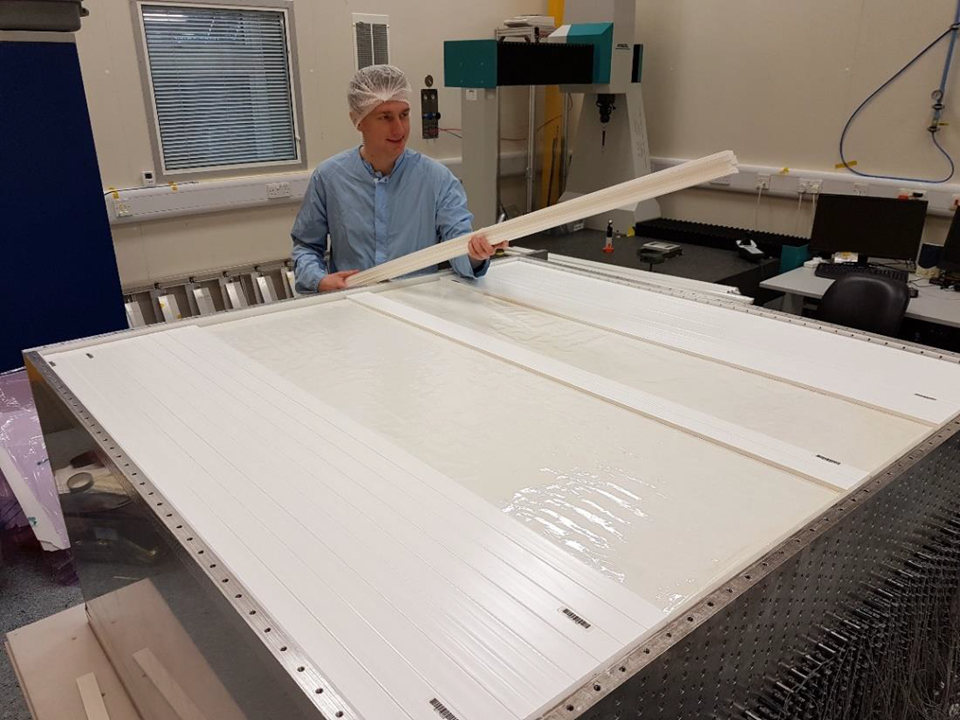
\includegraphics[width=0.7\linewidth]{Chapter3/Figs/Raster/detCon006_RonInCleanRoom.png}
\captionof{figure}[The author assembling the final layer of the VIDARR detector.]{The author (Ronald Collins) assembling the final layer of the VIDARR detector. The white sheet of Gadolinium Oxide in-between the layers is also visible.} 
\label{fig:detCon006_RonInCleanRoom}
\end{figure}

\begin{figure}[!h]
\centering
\begin{subfigure}{.5\textwidth}
  \centering
  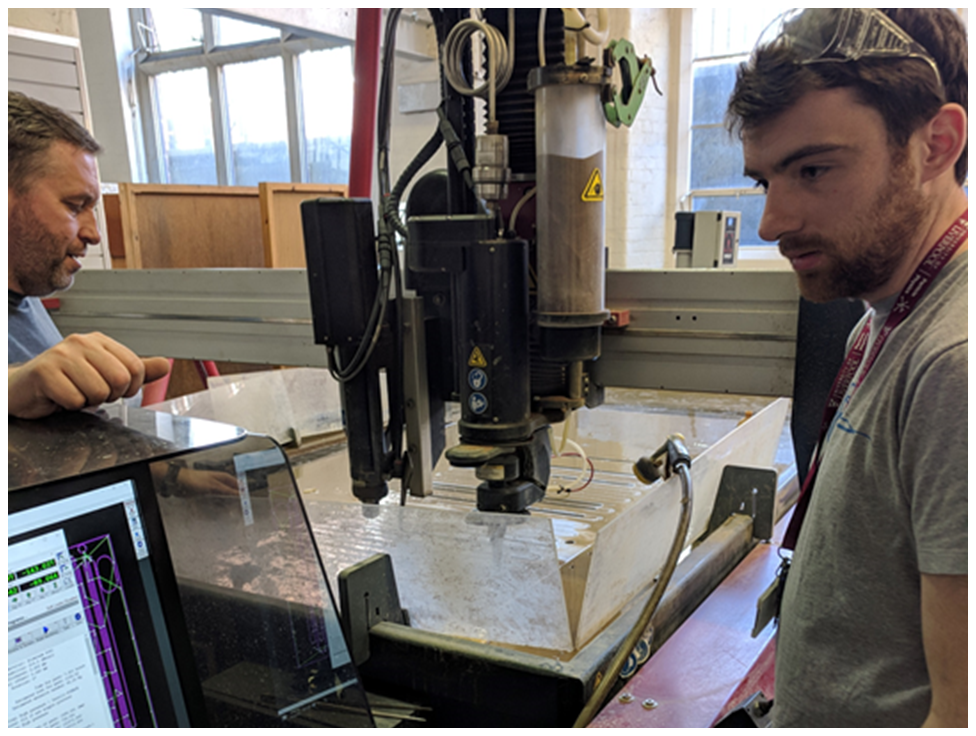
\includegraphics[width=\linewidth]{Chapter3/Figs/Raster/detCon011b_RadiatorConstruction.png}
  \captionsetup{width=.9\linewidth}
  \caption{}
  \label{subFig:detCon011b_RadiatorConstruction}
\end{subfigure}%
\begin{subfigure}{.5\textwidth}
  \centering
  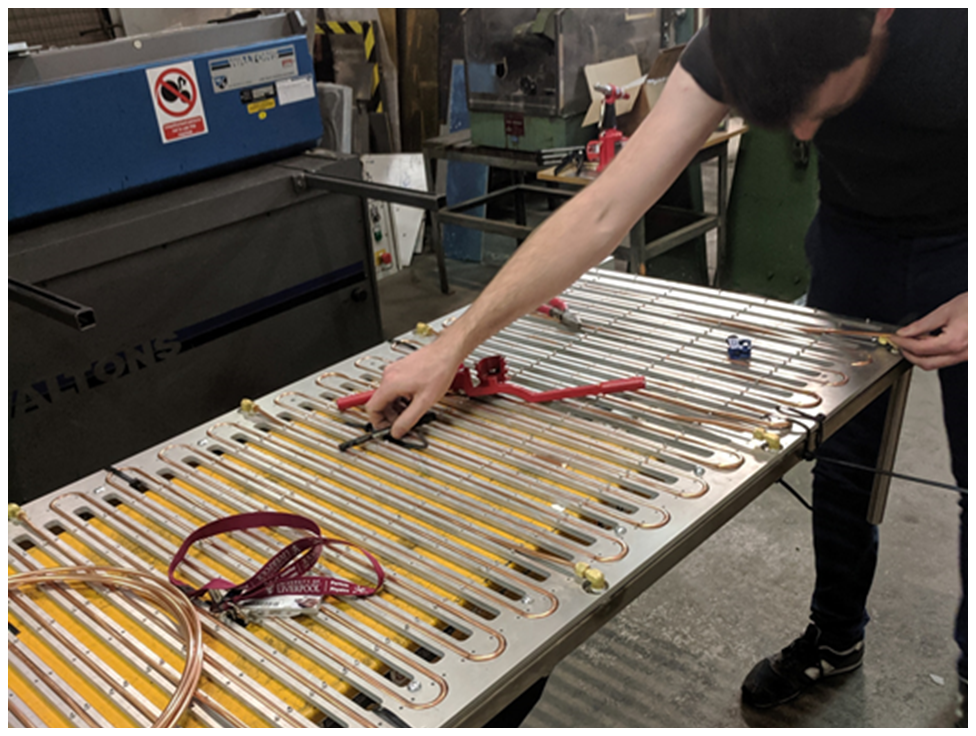
\includegraphics[width=\linewidth]{Chapter3/Figs/Raster/detCon012b_RadiatorPiping.png}
  \captionsetup{width=.9\linewidth}
  \caption{}
  \label{subFig:detCon012b_RadiatorPiping}
\end{subfigure}
\caption[Construction of the new more massive radiator.]{The construction of the new radiator which has more active cooling and a larger surface area than the original radiator. The radiator is being cut in (a) and the piping is inserted in (b).}
\label{fig:detCon_RadiatorConstruction_RadiatorPiping}
\end{figure}

The upgraded electronics for VIDARR draw more power and require substantially more cooling than the ECal electronics, and major improvements were made to cool the temperature sensitive MPPCs and thermally isolate them from the electronics. The original detector had much space between the electronic boards and the MPPCs with the electronic boards placed directly on cooling fins (see in figure \ref{fig:detCon002_OldTearAway}). In addition to the cooling fins seen in figure \ref{fig:detCon002_OldTearAway}, large radiators have now been added between the cooling fins and the MPPCs for each side. These new radiators are comprised of large stainless steel plates which were water-jet cut as shown in figure \ref{subFig:detCon011b_RadiatorConstruction}. Then copper piping was placed in the channels seen in figure \ref{subFig:detCon012b_RadiatorPiping}. This copper piping will face the MPPCs and the detector scintillator whilst the radiator fins will be attached behind the radiator away from the MPPCs and behind a 1\,cm thick (in X) layer of insulation. As in the prototype, the electronic boards will be placed on the fins similar to figure \ref{fig:detCon002_OldTearAway}. This will improve the cooling in the detector significantly and provide the isolation between the electronics boards and the scintillator and the MPPCs when compared to the Wylfa detector. 

% Once the scintillator is in the detector casing several individual components need to be assembled so that the light emitted by the scintillator can then be analysed. A small amount of light emitted by the scintillator upon particle interaction is trapped by the WLS fibres . These fibres are threaded through the centre of the scintillator and capture light and shift it to green light seen in figure \ref{subFig:detCon013b_WlsFibres}. These WLS fibres then have 3D printed connectors glued to the ends of them as seen in figure \ref{subFig:detCon014b_WlsWithEnds}. 3D printing was done as more vacuum moulded parts couldn't be obtained from the original supply chain which RMon used. The 3D printing was done by a Formlabs Form2 resin printer, the components were similar in quality but slightly more brittle and much easier to obtain.

Before insertion into the scintillator bars, the wavelength shifting fibres needed to be connected to aid the transport of wavelength shifted scintillation light to the MPPCs. Ferrules were glued to one end of each fibre. These parts were originally injection moulded, however due to problems with the supply chain, the majority of the new stock were 3D printed using a Formlabs Form2 resin printer. The ease of manufacture outweighed the disadvantage of slightly more brittle components. The fibres with and without ferrules attached are shown in figure \ref{fig:detCon_WlsFibres_WlsWithEnds}. The WLS fibres were also then painted with TiO$_2$ to improve light output. Then the MPPCs connectors are 3D printed seen both with the 3D-printing supports in figure \ref{subFig:detCon015b_3dPrintedHolders} and without in figure \ref{subFig:detCon016b_3dPrintedFreed}. The holders for the MPPCs were also 3D printed. These connect with the WLS fibres, aligning the output of the fibre onto the MPPC sensor as well as providing a mounting point for mini-PCBs which electronically connect to the terminals of the MPPCs. A sheet of which can be seen in figure \ref{subFig:detCon008b_PlacingPcbs}. These PCBs have to have a micro-coaxial cable connector soldered on to them and have through-hole connections for the MPPCs. A finished example of one of these PCBs can be seen in figure \ref{subFig:detCon009b_SoloPcb}. The holders, PCBs, and MPPCs all connect together as shown in figure \ref{fig:detCon017b_HoldersWithParts}. 

\begin{figure}[!h]
\centering
\begin{subfigure}{.5\textwidth}
  \centering
  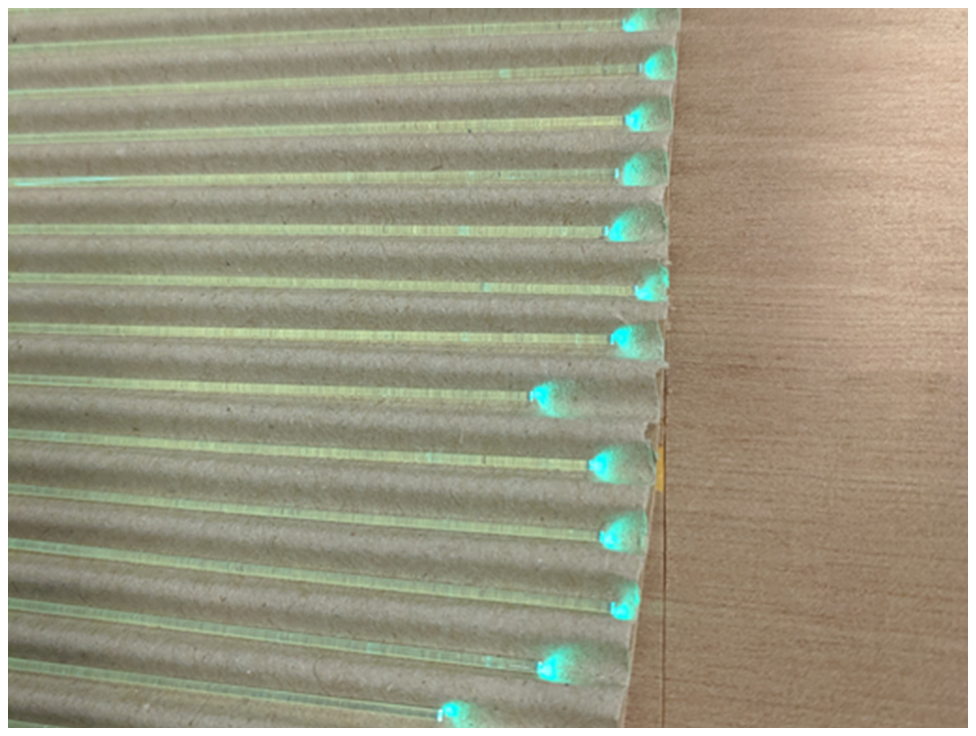
\includegraphics[width=\linewidth]{Chapter3/Figs/Raster/detCon013b_WlsFibres.png}
  \captionsetup{width=.9\linewidth}
  \caption{}
  \label{subFig:detCon013b_WlsFibres}
\end{subfigure}%
\begin{subfigure}{.5\textwidth}
  \centering
  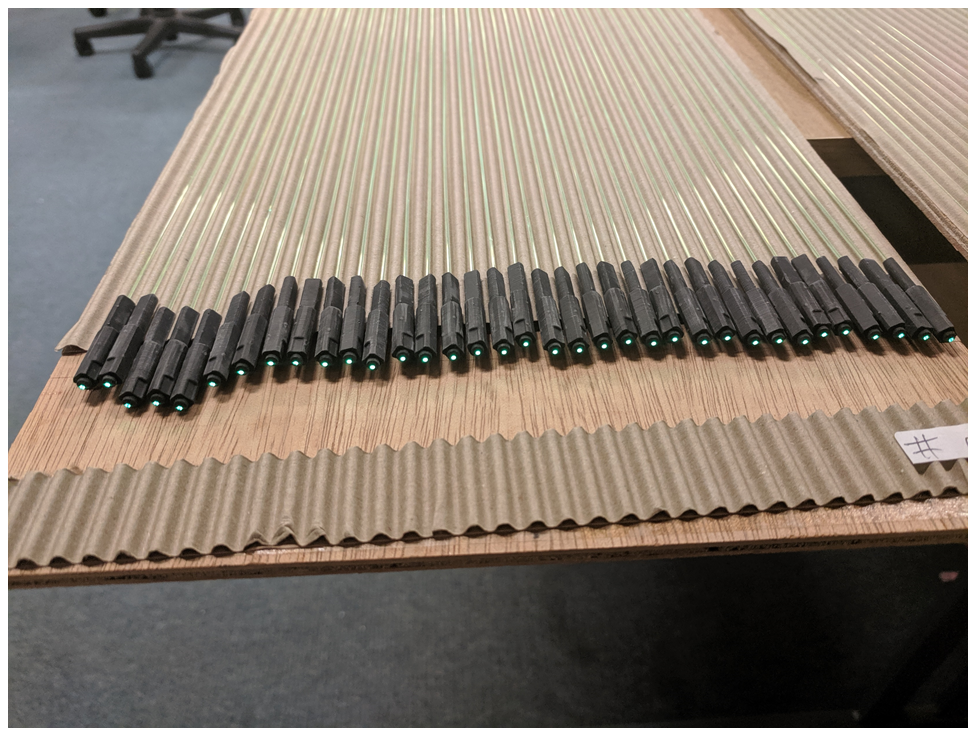
\includegraphics[width=\linewidth]{Chapter3/Figs/Raster/detCon014b_WlsWithEnds.png}
  \captionsetup{width=.9\linewidth}
  \caption{}
  \label{subFig:detCon014b_WlsWithEnds}
\end{subfigure}
\caption[WLS fibres having their ferrules attached.]{The WLS fibres. In (a) they are laid down on cardboard guides in (b) their ferrules are attached. The green light emitted at the ends of the fibre is ambient light wavelength shifted and channelled towards the end by the fibres.} %The WLS fibres will funnel light from the scintillator to the MPPCs. They are assembled on cardboard and have 3d printed ends glued onto them. In (a) the WLS fibres are prepared for their ends by lying on cardboard. In (b) the ends have been glued on.
\label{fig:detCon_WlsFibres_WlsWithEnds}
\end{figure}

\begin{figure}[!h]
\centering
\begin{subfigure}{.5\textwidth}
  \centering
  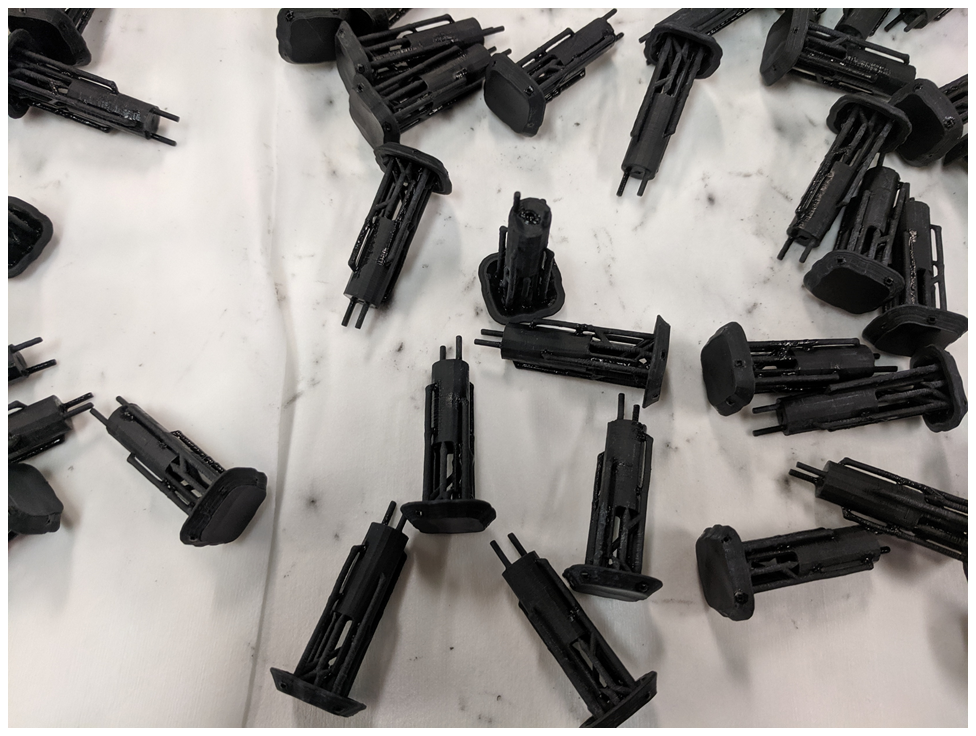
\includegraphics[width=\linewidth]{Chapter3/Figs/Raster/detCon015b_3dPrintedHolders.png}
  \captionsetup{width=.9\linewidth}
  \caption{}
  \label{subFig:detCon015b_3dPrintedHolders}
\end{subfigure}%
\begin{subfigure}{.5\textwidth}
  \centering
  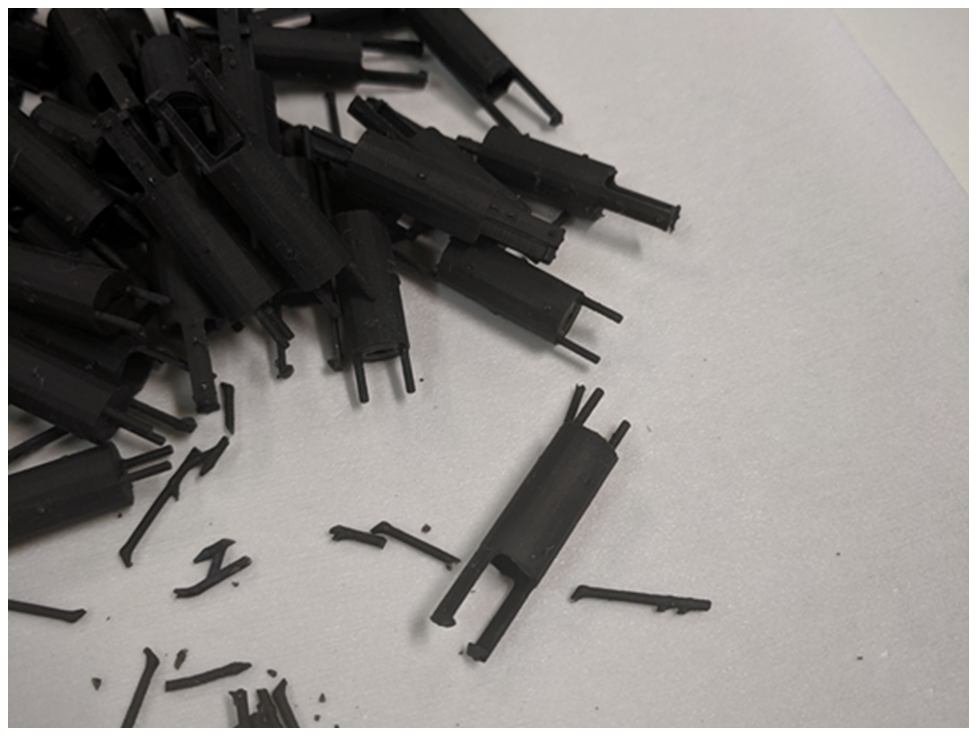
\includegraphics[width=\linewidth]{Chapter3/Figs/Raster/detCon016b_3dPrintedFreed.png}
  \captionsetup{width=.9\linewidth}
  \caption{}
  \label{subFig:detCon016b_3dPrintedFreed}
\end{subfigure}
\caption[The holders for the MPPCs and the PCBs]{The holders for the MPPCs and the PCBs. Holders for the additional channels needed to be 3D printed as more from the original supply chain could not be procured. In (a) the holders have the support struts attached and in (b) they have been removed.}
\label{fig:detCon_3dPrintedHolders_3dPrintedFreed}
\end{figure}

\begin{figure}[!h]
\centering
\begin{subfigure}{.5\textwidth}
  \centering
  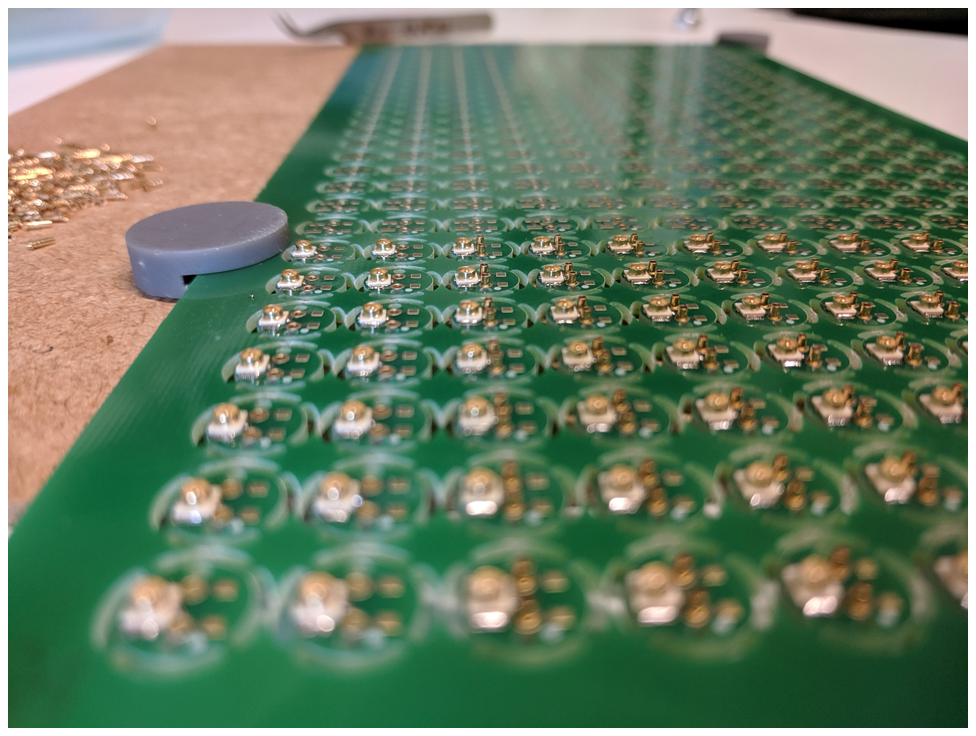
\includegraphics[width=\linewidth]{Chapter3/Figs/Raster/detCon008b_PlacingPcbs.png}
  \captionsetup{width=.9\linewidth}
  \caption{}
  \label{subFig:detCon008b_PlacingPcbs}
\end{subfigure}%
\begin{subfigure}{.5\textwidth}
  \centering
  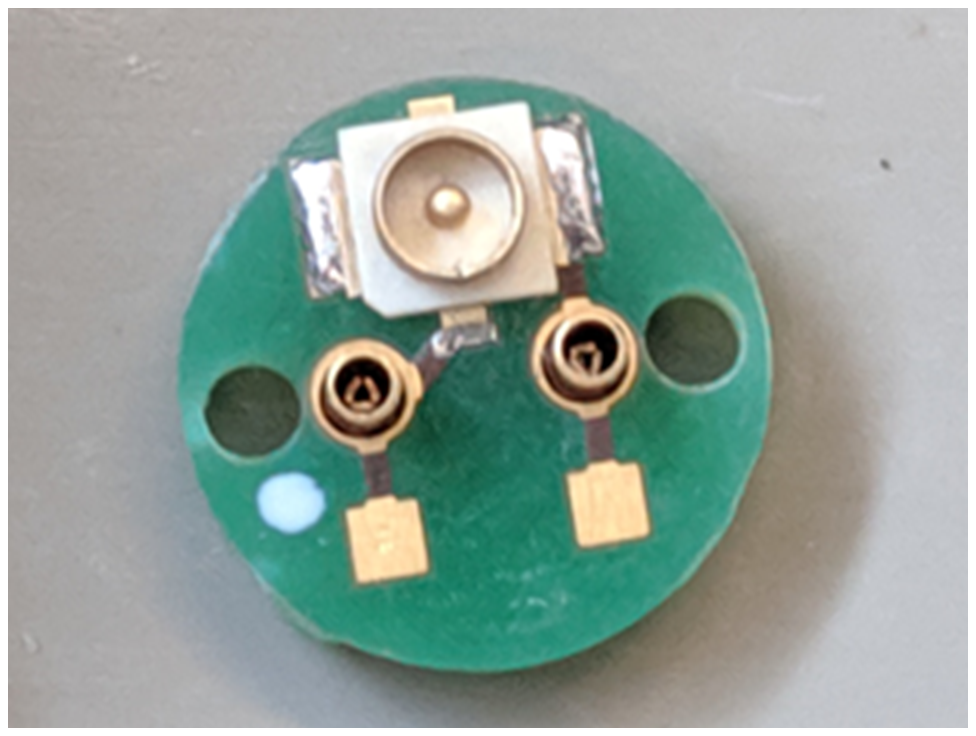
\includegraphics[width=\linewidth]{Chapter3/Figs/Raster/detCon009b_SoloPcb.png}
  \captionsetup{width=.9\linewidth}
  \caption{}
  \label{subFig:detCon009b_SoloPcb}
\end{subfigure}
\caption[Assembly of the MPPC PCBs.]{The assembly of the PCBs which attach to the MPPCs through pins. (a) shows a sheet of manufactured incomplete PCBs and (b) shows a completed component. The connector at the top of the PCBs is where the cables are attached. }
\label{fig:detCon_PlacingPcbs_SoloPcb}
\end{figure}

Each of the micro-coaxial cables that connect the MPPCs to the analogue boards were labelled with heat shrink labels to ensure the labels were secure. The label syntax is side-row-column with the bottom left of each side being the coordinate for (0,0). An example of this syntax would be B-10-37 indicating side B row 10 and column 37. These labels were then slid onto the micro-coaxial cables 8\,cm from the end that connects to the analogue boards and heat shrunk. These cables were then connected to the holders where the PCB connector seen in figure \ref{subFig:detCon009b_SoloPcb} connects firmly to the cable. The holder was also put into a sheath so that was held firmly in place once inside the detector, as seen in figure \ref{fig:detCon023b_HoldersConnectedZoom}.

\begin{figure}[!h]
\centering
\begin{minipage}{.45\textwidth}
  \centering
  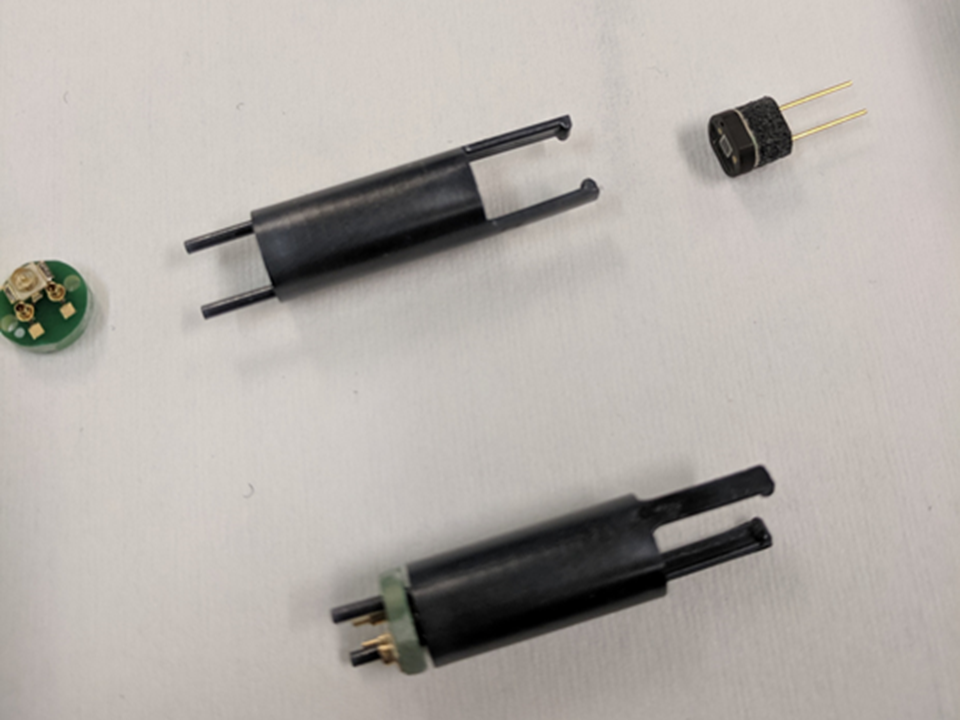
\includegraphics[width=\linewidth]{Chapter3/Figs/Raster/detCon017b_HoldersWithParts.png}
  \captionof{figure}[Plastic holder for the MPPC next to the MPPC.]{Plastic holder next to MPPC and PCB (Top) and holder with assembled components (Bottom). Note the MPPC in the top right is actually reversed from its correct orientation, the prongs of the MPPC go through the PCB board pins.} 
  \label{fig:detCon017b_HoldersWithParts}
\end{minipage}%
\qquad
\begin{minipage}{.45\textwidth}
  \centering
  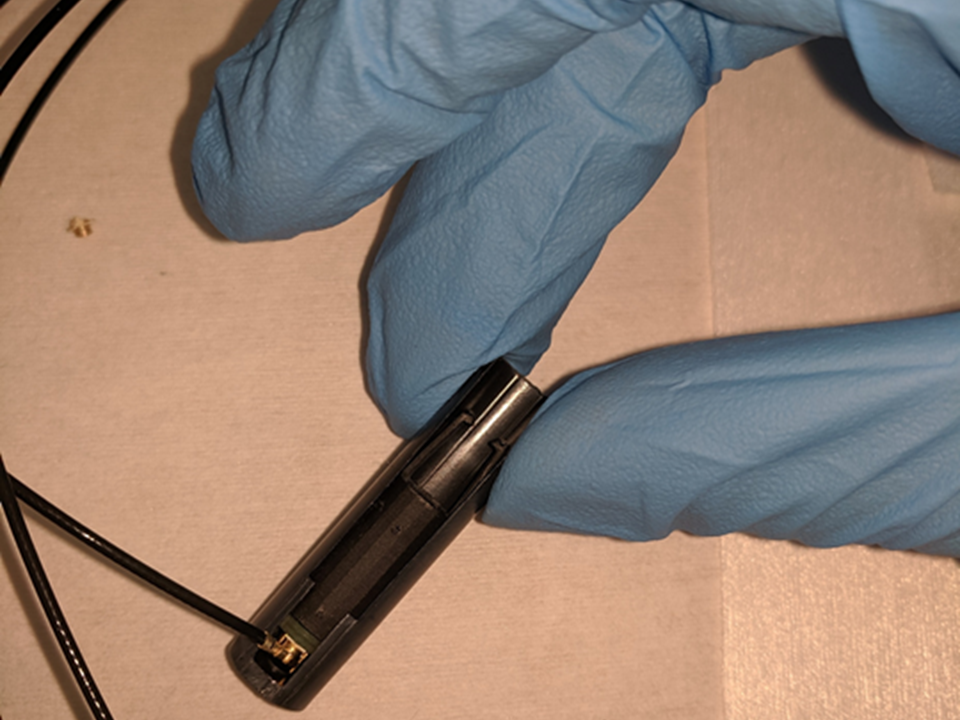
\includegraphics[width=\linewidth]{Chapter3/Figs/Raster/detCon023b_HoldersConnectedZoom.png} 
  \captionof{figure}[Plastic holder connected to a cable and put inside a sheath.]{The plastic holder is connected to a cable and put inside a sheath.}
  \label{fig:detCon023b_HoldersConnectedZoom}
  \vspace{1.912cm} %1 line = 0.478cm % 2 lines = 0.956cm % 3 lines= 1.434cm % 4 lines = 1.912cm % 5 lines = 2.39cm
\end{minipage}
\end{figure}

% \begin{figure}[!h]
% \centering
% \begin{subfigure}{.5\textwidth}
%   \centering
%   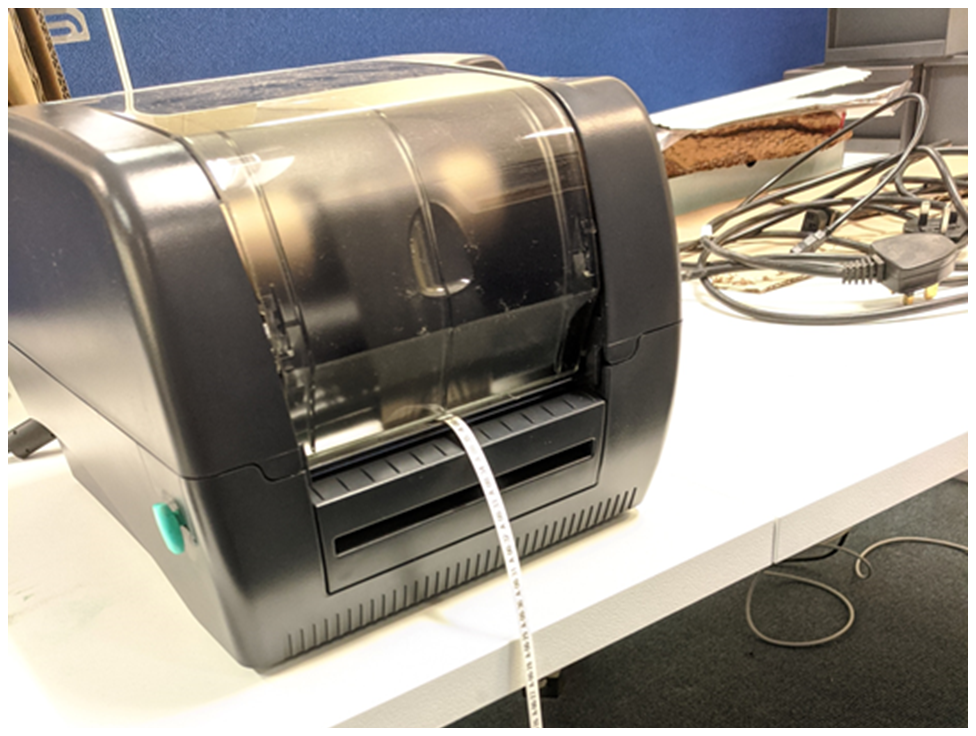
\includegraphics[width=\linewidth]{Chapter3/Figs/Raster/detCon018b_HeatLabelsPrinted.png}
%   \captionsetup{width=.9\linewidth}
%   \caption{Heat shrink labels being printed out.}
%   \label{subFig:detCon018b_HeatLabelsPrinted}
% \end{subfigure}%
% \begin{subfigure}{.5\textwidth}
%   \centering
%   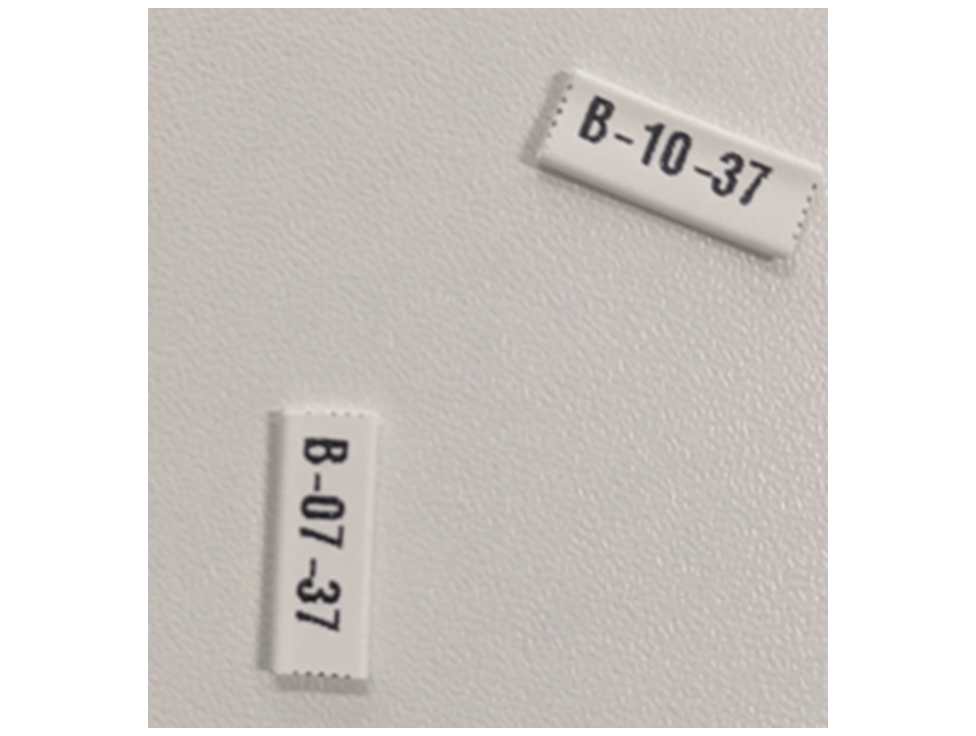
\includegraphics[width=\linewidth]{Chapter3/Figs/Raster/detCon019b_CutLabels.png}
%   \captionsetup{width=.9\linewidth}
%   \caption{Individual labels for specific cables.}
%   \label{subFig:detCon019b_CutLabels}
% \end{subfigure}
% \caption{Heat-shrink labels are used to identify cables. Labels are printed out in the form side-Row-Column where the bottom left is (0,0) }
% \label{fig:detCon_HeatLabelsPrinted_CutLabels}
% \end{figure}

% \begin{figure}[!h]
% \centering
% \begin{subfigure}{.5\textwidth}
%   \centering
%   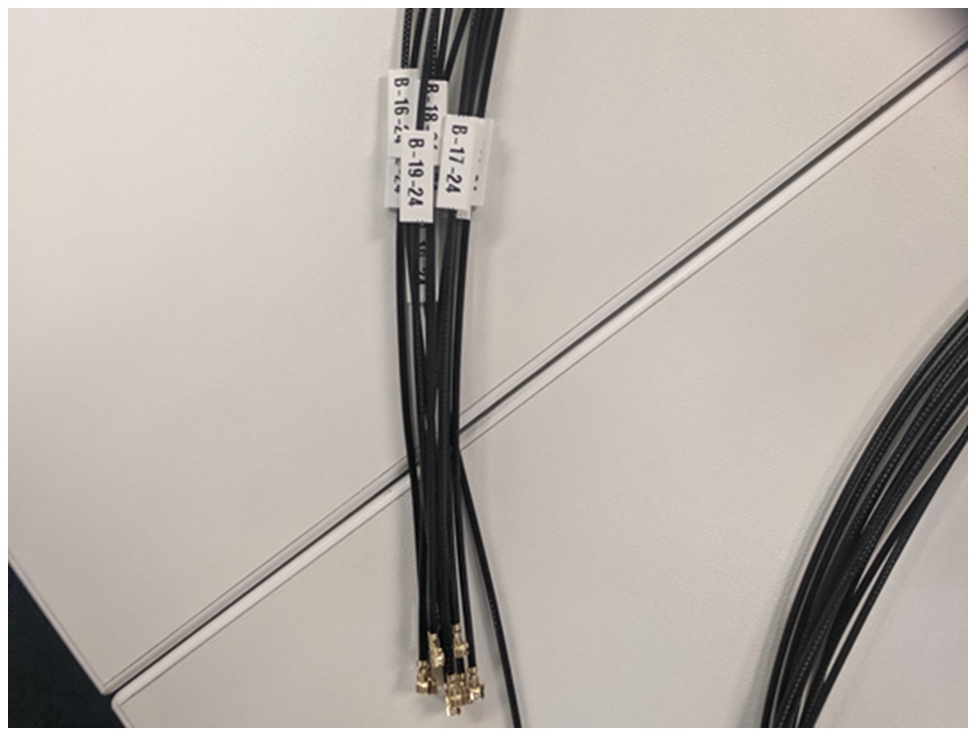
\includegraphics[width=\linewidth]{Chapter3/Figs/Raster/detCon020b_LabelsLoose.png}
%   \captionsetup{width=.9\linewidth}
%   \caption{}
%   \label{subFig:detCon020b_LabelsLoose}
% \end{subfigure}%
% \begin{subfigure}{.5\textwidth}
%   \centering
%   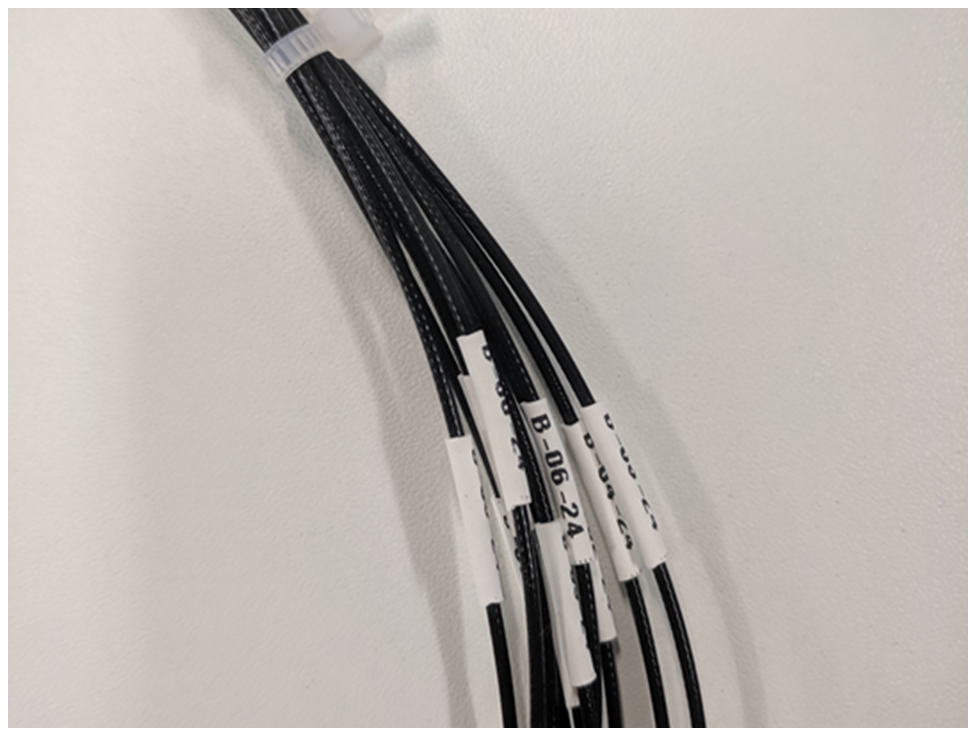
\includegraphics[width=\linewidth]{Chapter3/Figs/Raster/detCon021b_LabelsHeated.png}
%   \captionsetup{width=.9\linewidth}
%   \caption{}
%   \label{subFig:detCon021b_LabelsHeated}
% \end{subfigure}
% \caption{Labels are threaded through at 8\,cm from the end of the cables as seen in (a) then a heat gun is used on the cables to shrink the labels and they are bunched as seen in (b).}
% \label{fig:detCon_LabelsLoose_LabelsHeated}
% \end{figure}

All of the MPPC holders in their sheaths with connected cables are then attached to the WLS fibres and their 3D printed connectors shown in figure \ref{subFig:detCon014b_WlsWithEnds}. There are two distinct sheath types: grey made via injection moulding and orange sheaths which were 3D printed. These sheaths protect the rest of the components and can be seen clearly in figure \ref{fig:detCon_HaningOffRadiator_RadiatorTopDown} as they protrude from the detector casing. The radiator was slowly moved into position as cables were threaded through the insulation layer as can be seen in figure \ref{subFig:detCon026b_HaningOffRadiator}. Once the radiator was moved into position, the space between the radiator and sheaths was checked to ensure that no undue pressure was being applied to the sheaths (figure \ref{subFig:detCon028b_RadiatorTopDown}). Once the radiator was in position, the cooling fins were  attached as (figure \ref{fig:detCon030b_RadiatorWithFins}). Cross-shaped base-plate board holders are then screwed into cooling fins (figure \ref{fig:detCon030b_RadiatorWithFins}) with thermal paste between the fins and and base-plates to counteract any lack of contact between the base-plates and the cooling fins. An example of how the analogue processing boards (APB) are attached to the cooling fins can be seen in figure \ref{fig:detCon032_ConnectedBoard}. This figure also how the cables are connected to the APB and aligned through an orange cable comb. To aid cooling, a $5\,\textrm{cm}\times5\,\textrm{cm}$ thermal pad will be placed between the base-plate and the APB. Then ADC mezzanine boards (AMB) will connect to the APBs. The AMB connected to the top of the APB will be air cooled, with heat generating components (ADCs, FPGA) mounted with heat sinks.

\begin{figure}[!h]
\centering
\begin{subfigure}{.5\textwidth}
  \centering
  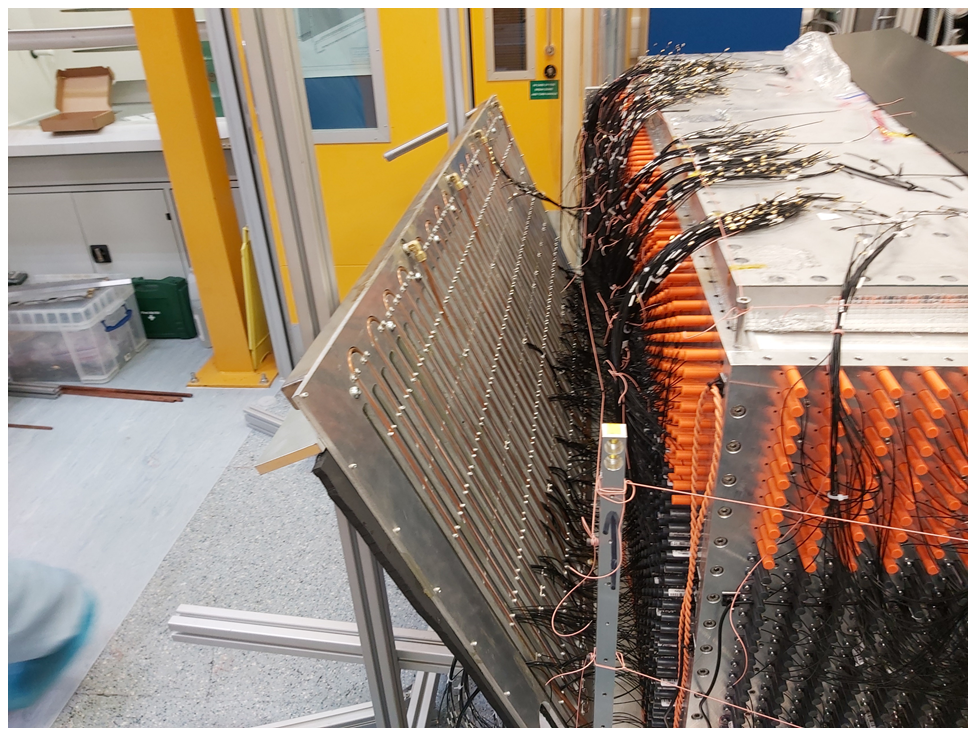
\includegraphics[width=\linewidth]{Chapter3/Figs/Raster/detCon026b_HaningOffRadiator.png}
  \captionsetup{width=.9\linewidth}
  \caption{}
  \label{subFig:detCon026b_HaningOffRadiator}
\end{subfigure}%
\begin{subfigure}{.5\textwidth}
  \centering
  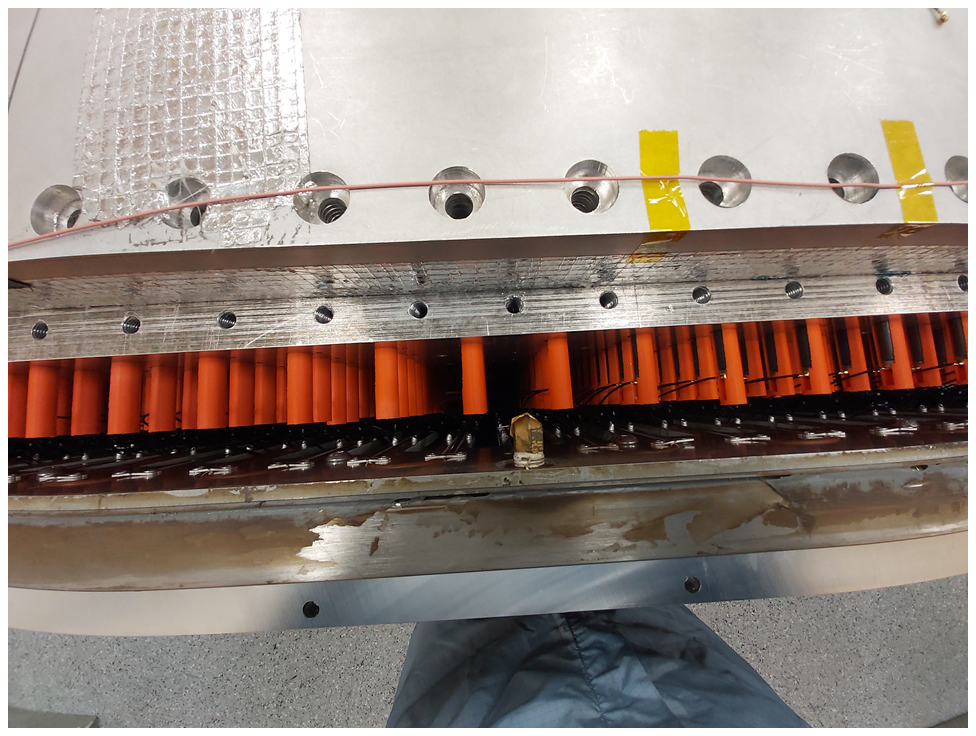
\includegraphics[width=\linewidth]{Chapter3/Figs/Raster/detCon028b_RadiatorTopDown.png}
  \captionsetup{width=.9\linewidth}
  \caption{}
  \label{subFig:detCon028b_RadiatorTopDown}
\end{subfigure}
\caption[The new more massive radiators being put into position.]{As part of the upgrade, the radiators are significantly larger ensuring the MPPCs are closer to the radiator. In (a) the side A radiator is positioned as the cables are threaded through the insulation on the radiator. In (b) the side A radiator is now in position with all the cables threaded through the insulation.}
\label{fig:detCon_HaningOffRadiator_RadiatorTopDown}
\end{figure}

% \begin{figure}[!h]
% \centering
% \begin{subfigure}{.5\textwidth}
%   \centering
%   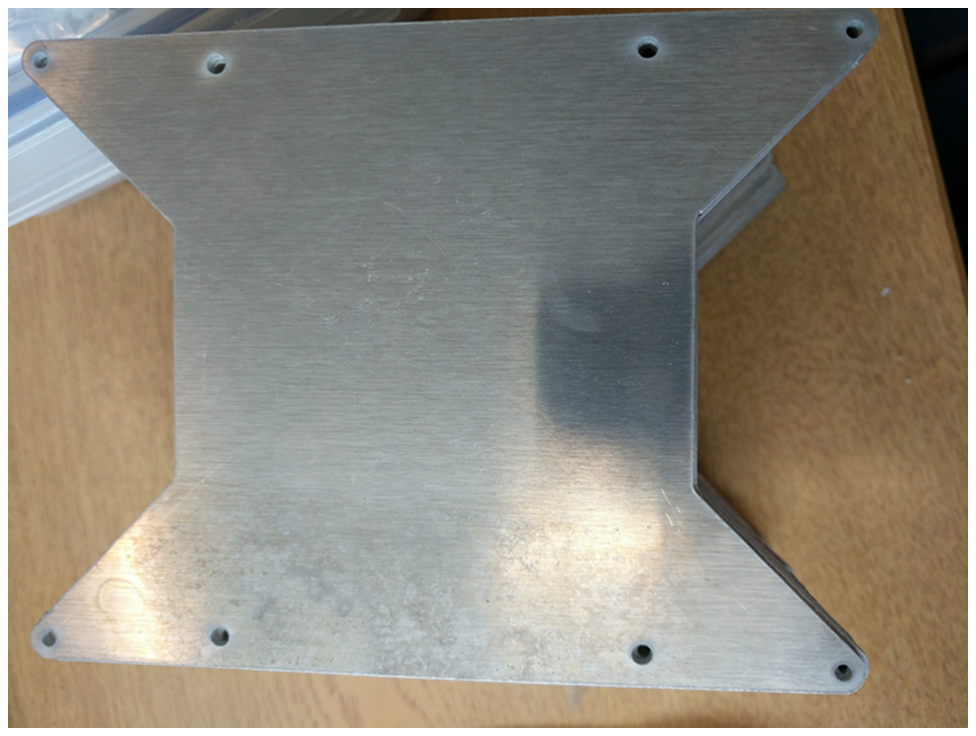
\includegraphics[width=\linewidth]{Chapter3/Figs/Raster/detCon029b_coolantFin.png}
%   \captionsetup{width=.9\linewidth}
%   \caption{Board holders that connect the analogue boards to the cooling fins.}
%   \label{subFig:detCon029b_coolantFin}
% \end{subfigure}%
% \begin{subfigure}{.5\textwidth}
%   \centering
%   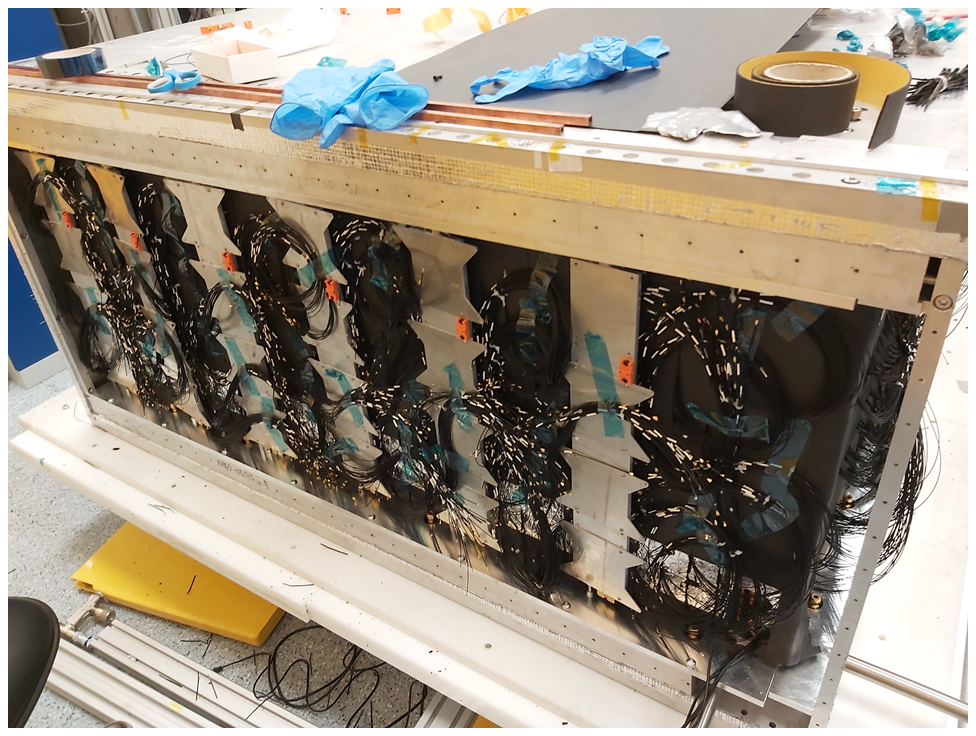
\includegraphics[width=\linewidth]{Chapter3/Figs/Raster/detCon030b_RadiatorWithFins.png}
%   \captionsetup{width=.9\linewidth}
%   \caption{Cooling fins and board holders attached to the radiator.}
%   \label{subFig:detCon030b_RadiatorWithFins}
% \end{subfigure}
% \caption{The analogue board holders and cooling fins are attached after the cables are threaded through the radiator insulation.}
% \label{fig:detCon_coolantFin_RadiatorWithFins}
% \end{figure}

\begin{figure}[!h]
\centering
\begin{minipage}{.45\textwidth}
  \centering
  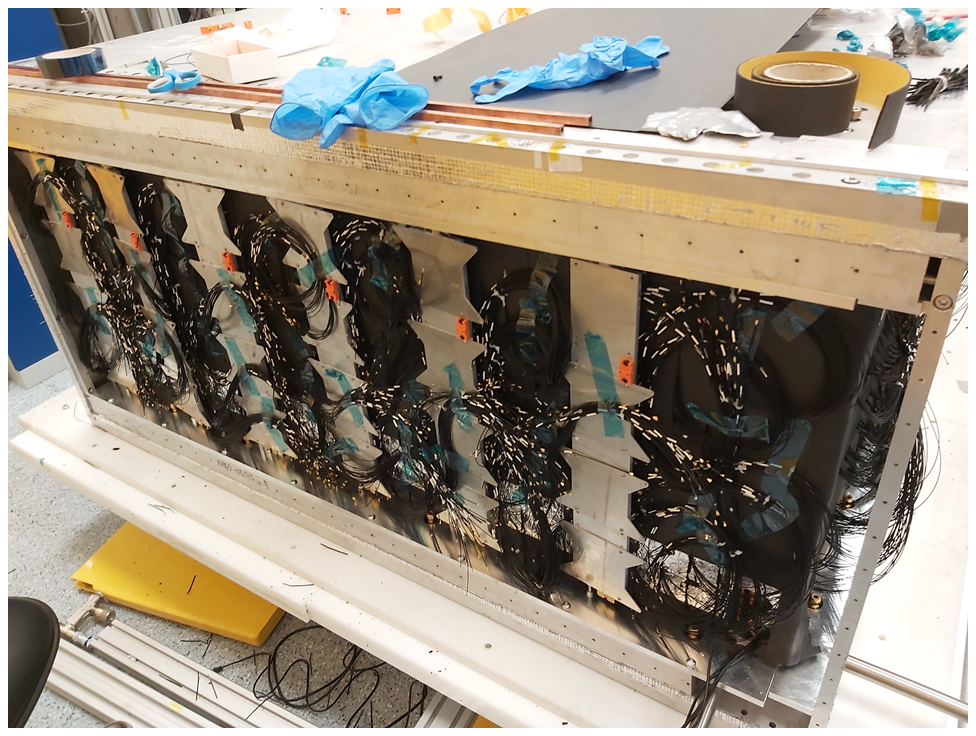
\includegraphics[width=\linewidth]{Chapter3/Figs/Raster/detCon030b_RadiatorWithFins.png}
  \captionof{figure}[The radiator attached to side A.]{The radiator on side A with the cooling fins and analogue board holders attached with cables pushed through the insulation and bunched.} 
  \label{fig:detCon030b_RadiatorWithFins}
\end{minipage}%
\qquad
\begin{minipage}{.45\textwidth}
  \centering
  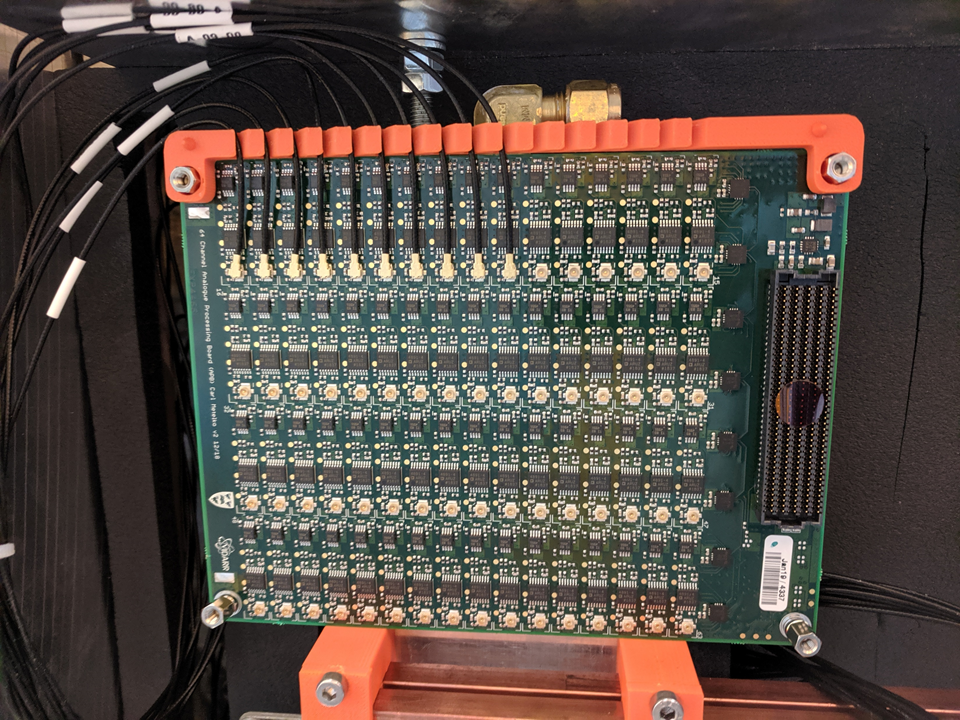
\includegraphics[width=\linewidth]{Chapter3/Figs/Raster/detCon032_ConnectedBoard.png} 
  \captionof{figure}[VIDARR analogue board with some cables connected.]{An analogue board with some of the cables connected to it. A 3D printed cable ``comb'' is used to align the cables.}
  \label{fig:detCon032_ConnectedBoard}
  \vspace{0.478cm} %1 line = 0.478cm % 2 lines = 0.956cm % 3 lines= 1.434cm % 4 lines = 1.912cm % 5 lines = 2.39cm
\end{minipage}
\end{figure}

The upgraded container, which can be seen in figure \ref{subFig:detCon037c_ContainerArrives}, was delivered in September 2019. The detector could not be moved into the container until all services especially air conditioning were installed and tested. The upgrade's progress ceased around the same time as the container arrived during September of 2019 as an issue with electronics was discovered. This issue has now been addressed and installation will be able to continue in the near future. This issue has been addressed and although access to the department and services are still somewhat limited by COVID-19 restrictions, the upgraded detector is expected to be completed in 2022. As of November 2020 the detector resides in the upgraded detector (see figure \ref{subFig:detCon039b_PutIn2}) ready for the installation of the front-end boards and initial tests with the new read out chain.

%Currently, this remains unresolved. Due to the issues in the electronics supply chain caused by the COVID-19 crisis and the small size of the VIDARR collaboration obtaining replacement electronics has been impossible up to September of 2021. Though in recent months there has been some movement in obtaining the relevant components. 

\begin{figure}[!h]
\centering
\begin{subfigure}{.5\textwidth}
  \centering
  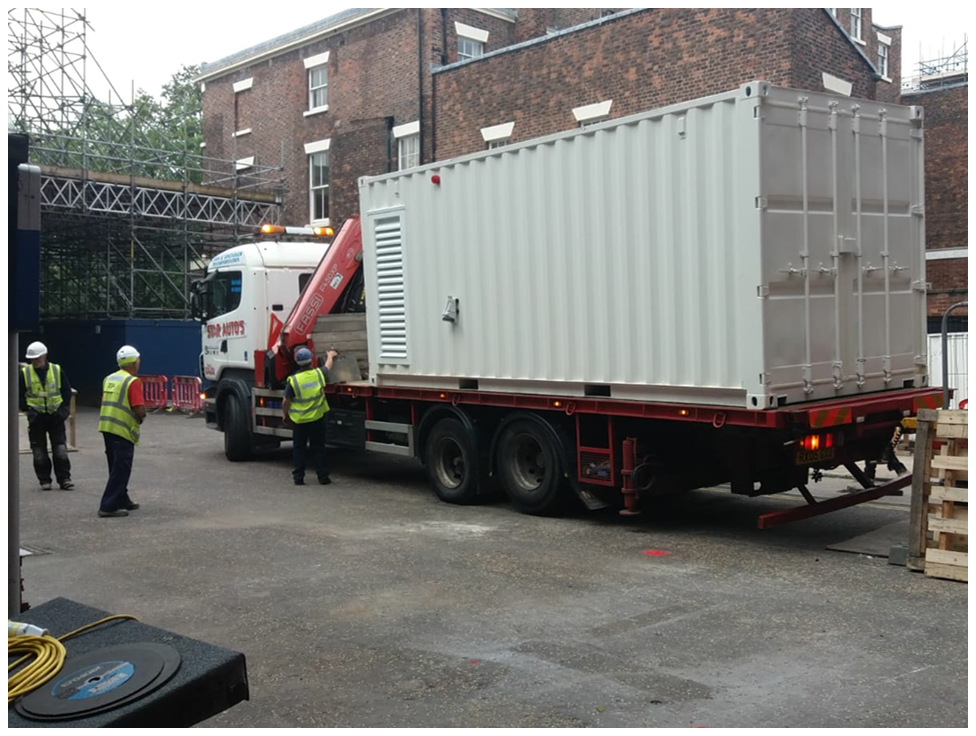
\includegraphics[width=\linewidth]{Chapter3/Figs/Raster/detCon037c_ContainerArrives.png}
  \captionsetup{width=.9\linewidth}
  \caption{}
  \label{subFig:detCon037c_ContainerArrives}
\end{subfigure}%
\begin{subfigure}{.5\textwidth}
  \centering
  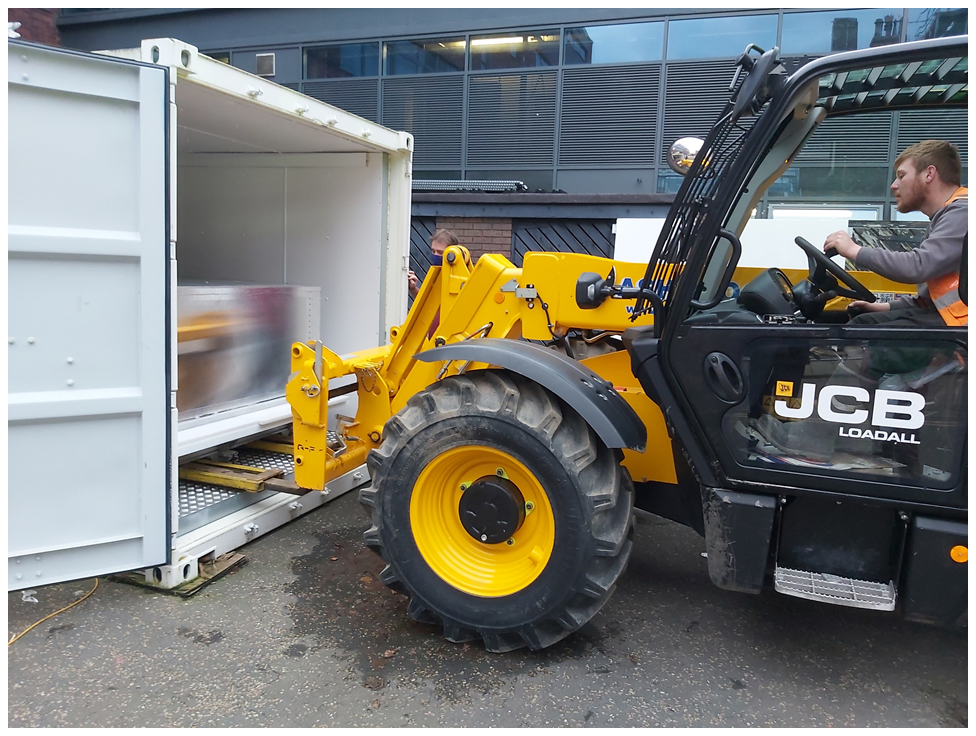
\includegraphics[width=\linewidth]{Chapter3/Figs/Raster/detCon039b_PutIn2.png}
  \captionsetup{width=.9\linewidth}
  \caption{}
  \label{subFig:detCon039b_PutIn2}
\end{subfigure}
\caption[The detector is deposited inside the new container.]{The new container arrives in (a) and the partially upgraded detector is deposited inside of it in (b).}
\label{fig:detCon_ContainerArrives_PutIn}
\end{figure}

% The detector upgrade has sadly stalled due to the COVID-19. Despite the unprecedented set back the VIDARR collaboration has still been able to increase the detector mass by $\sim$ 50\,\%, assemble and install new radiators, assemble new instruments, cable the MPPCs, and obtain a new container with cooling. Considering this it is reasonable to assume that the collaboration will be able to install the new electrons within good time. 

% The upgraded container has much improved airflow when compared to the original including air conditioning and an improved ventilation system. The upgraded container should be able to keep the temperature consistent and thus reduce the uncertainties caused by temperature fluctuations. In addition, there has been a significant improvement to computational power with an upgraded computer rack to read out detector information and a new computer with 64 total threads and 64\,GB of RAM to assist with analysis. Neither of these are currently in the container due to the issues with COVID-19 previously discussed as they are being used to diagnose any issues with the electronics and analyse older data sets.  

% \begin{figure}[!h]
% \centering
% 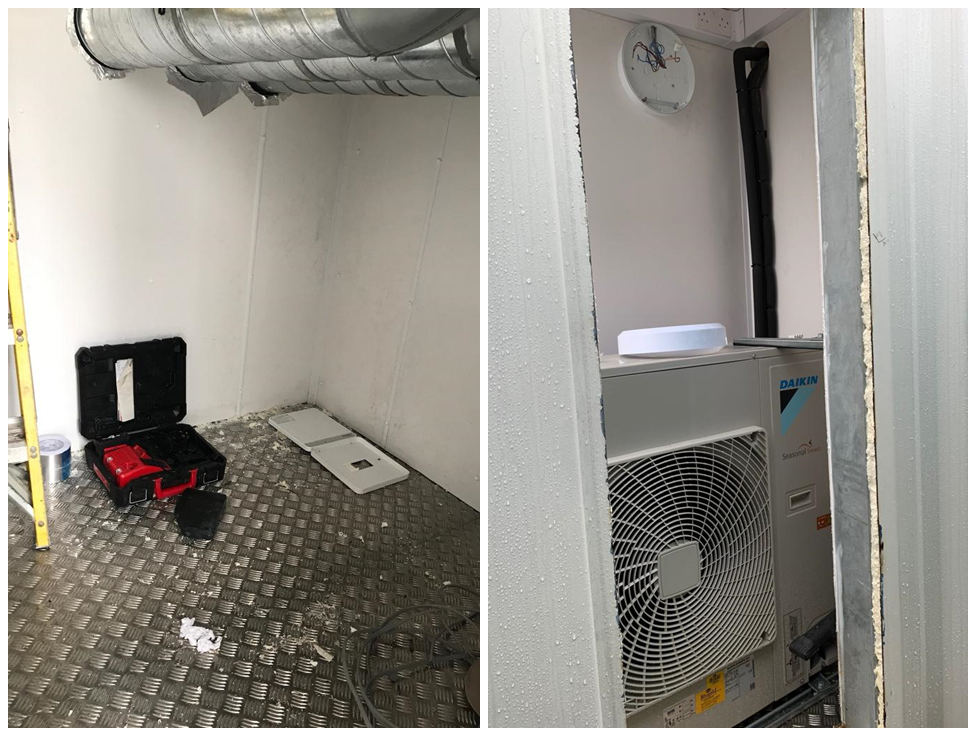
\includegraphics[width=0.7\linewidth]{Chapter3/Figs/Raster/detCon035b_ContainerAirCon.png}
% \captionof{figure}{The new container has air conditioning and an air circulatory system to help keep a consistent temperature.} 
% \label{fig:detCon035b_ContainerAirCon}
% \end{figure}

% \begin{figure}[!h]
% \centering
% 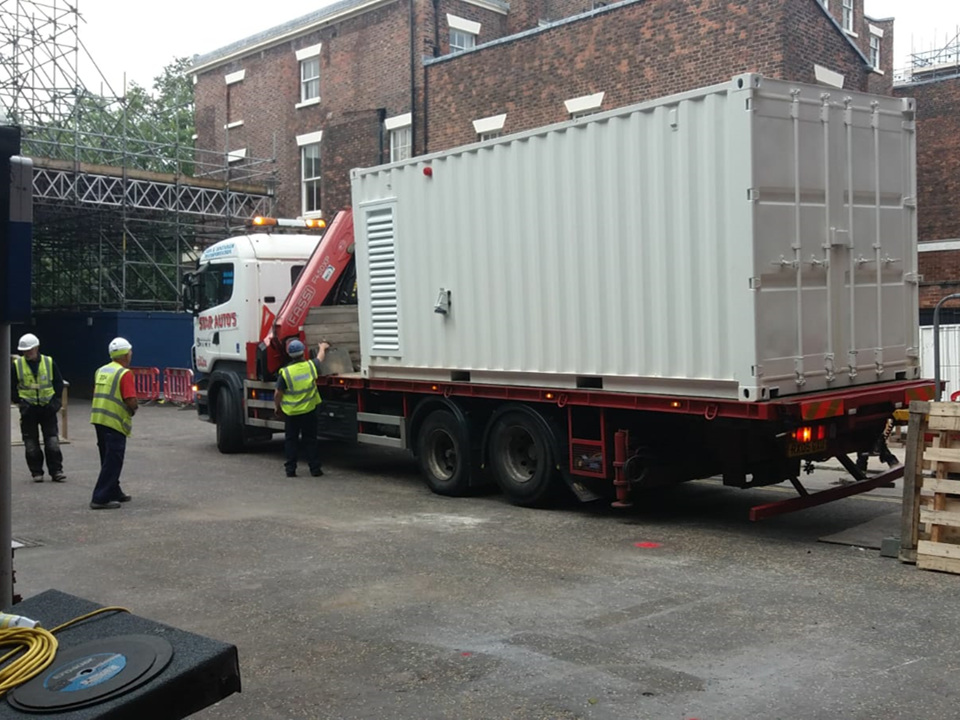
\includegraphics[width=0.8\linewidth]{Chapter3/Figs/Raster/detCon037b_ContainerArrives.png}
% \captionof{figure}{The new container arrives at the University of Liverpool.} 
% \label{fig:detCon037b_ContainerArrives}
% \end{figure}

% \begin{figure}[!h]
% \centering
% 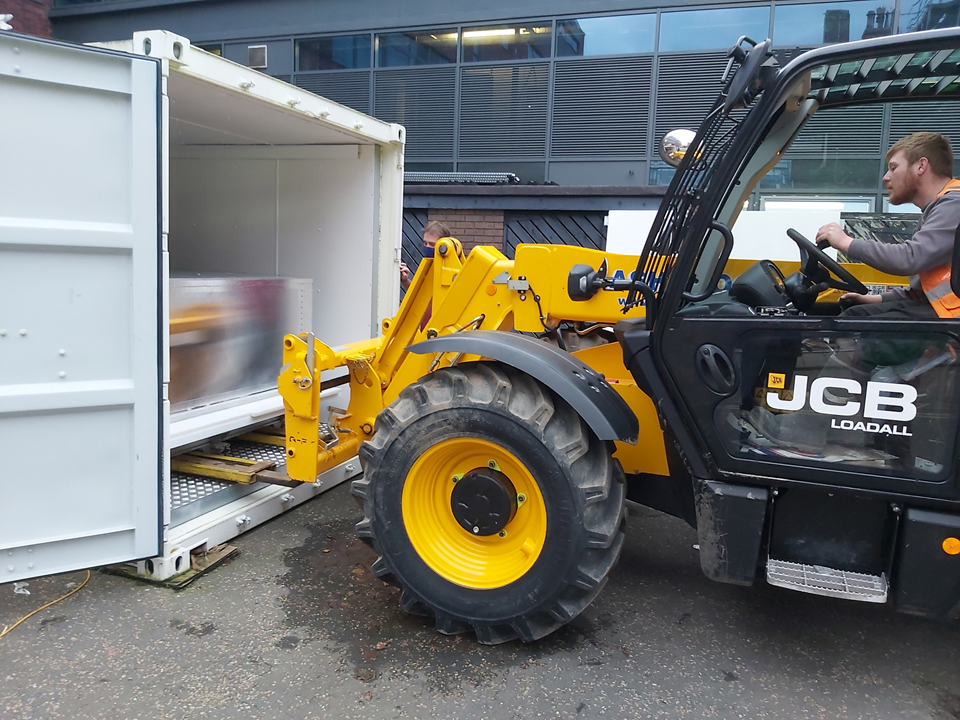
\includegraphics[width=0.8\linewidth]{Chapter3/Figs/Raster/detCon039_PutIn2.png}
% \captionof{figure}{The new detector being placed in the new container. (The upgrade was only partially completed at this time)} 
% \label{fig:detCon039_PutIn2}
% \end{figure}

% \begin{figure}[!h]
% \centering
% 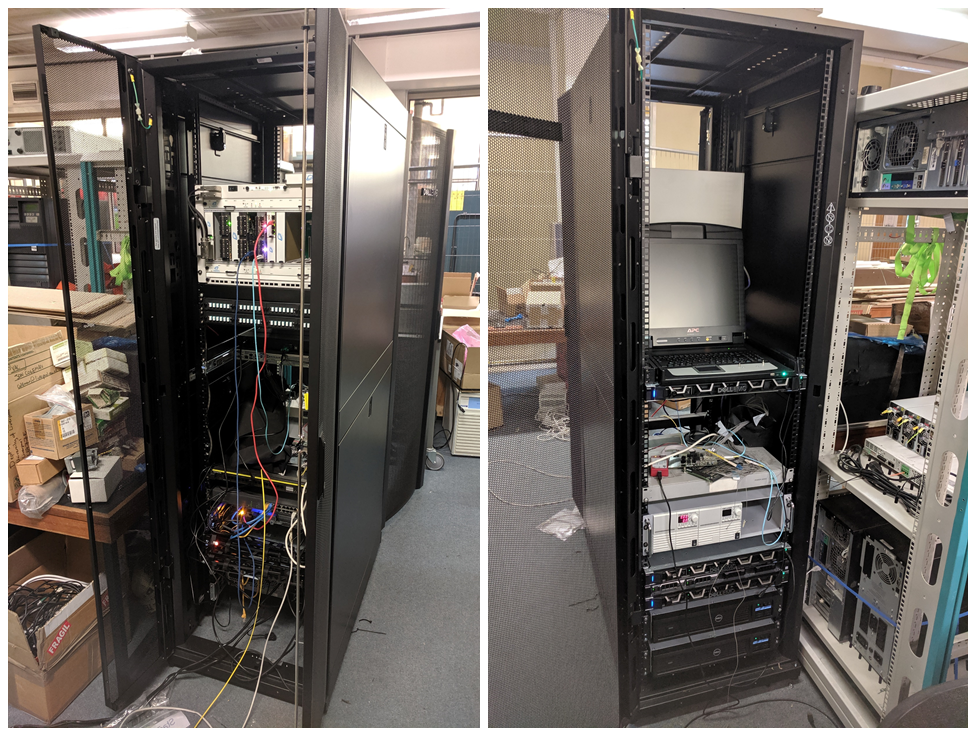
\includegraphics[width=0.7\linewidth]{Chapter3/Figs/Raster/detCon042b_Rack1.png}
% \captionof{figure}{The computer rack for the upgraded detector from the back (left) and front (right).} 
% \label{fig:detCon042b_Rack1}
% \end{figure}

% \begin{figure}[!h]
% \centering
% 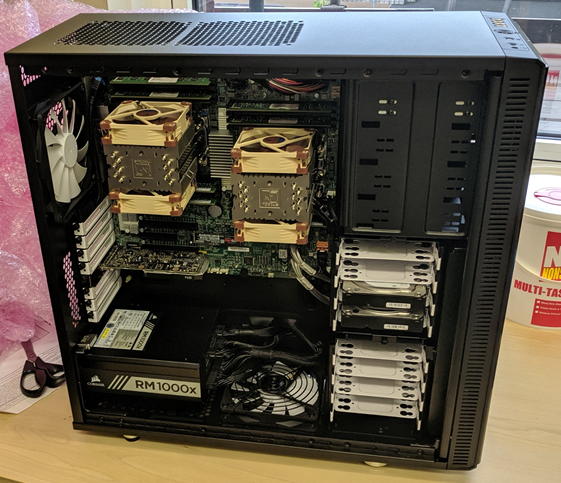
\includegraphics[width=0.8\linewidth]{Chapter3/Figs/Raster/detCon044_NewComputer.png}
% \captionof{figure}{The new computer for the upgraded detector. It has two 32 core CPUs and 64\,Gb of Ram.} 
% \label{fig:detCon044_NewComputer}
% \end{figure}

% \begin{figure}[!h]
% \centering
% 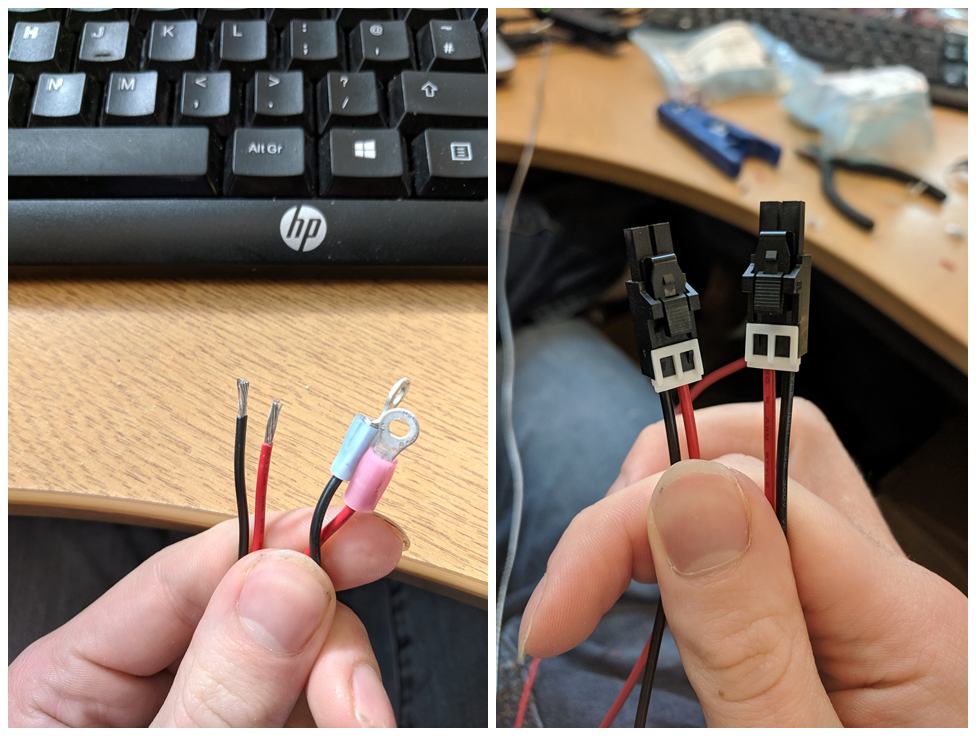
\includegraphics[width=0.7\linewidth]{Chapter3/Figs/Raster/detCon045b_PowerCabels1.png}
% \captionof{figure}{Power cables for the analogue boards that will attach to the central bus bars. \hl{may need to add some finer details remember to check with Carl}} 
% \label{fig:detCon045b_PowerCabels1}
% \end{figure}